\chapter{面向步态康复训练的主动膝关节矫形器交互式运动辅助轨迹规划生成}
基于机器人的步态训练已受到患者及临床医生的广泛认可。为实现这一目标,利用未受影响侧的运动数据生成受影响侧的参考轨迹成为一种重要手段。然而,在线生成步态参考轨迹需算法提供精确的步态相位延迟,同时降低传感器测量噪声及用户输入不确定性造成的影响。在本章中,研究基于一个自主开发的主动式膝关节矫形器原型样机,提出了一种适用于偏瘫患者步态康复的自适应对称步态轨迹生成框架。通过采用自适应非线性频率振荡器与节律动态运动基元,本章的研究实现了根据实时用户输入进行在线步态模式编码与自适应相位延迟。此外,进一步设计了具有在线输入验证与仲裁功能的共享自主框架,以避免来自健侧膝关节的不确定性运动导致的机器人轨迹规划生成安全性问题。通过一系列实验表明,所提出方法具备良好的可行性,且可以有效地防止用户或传感器输入噪声导致的辅助轨迹错误规划。

\section{研究动机与交互不确定性分析}
目前在我国中风现在仍然是一个严峻的公共卫生问题,现有患者数量庞大且逐年上升。据统计,我国中风患者数量达到了1494万人,每年有330万新发病例出现,而导致死亡的案例高达154万,占总死亡人数的22\%。在中风幸存者中,大约75\%遭受了不同程度的残疾影响,其中有40\%属于重度残疾。中风的高发年龄段主要是45岁以上的人群,65岁以上的人群尤其高发,而75岁以上患者的发病率是45至54岁人群的5到8倍。此外,中风给中国社会和家庭带来了巨大的经济负担,每年用于治疗的费用超过200亿元。中风具有高发病率和高致残率的特点,其中大多数中风患者都存在不同程度的步态障碍。在中风急性期,近70\% 患者存在行走障碍。即使康复并自然恢复,50 \% 偏瘫患者仍不能独立行走\cite{jorgensenRecoveryWalkingFunction1995}。步行能力的下降增加了患者二次伤害的风险,这严重影响了他们的生活质量\cite{balabanGaitDisturbancesPatients2014,yelnikClinicalGuideAssess1999}。步态对称性康复已成为中风患者康复的关键目标之一。近年来,来自国内外的多项研究已针对偏瘫患者的膝关节运动时空差异进行了深入探讨。大量研究结果表明,在下肢患侧的膝关节在整个站立阶段的大部分时间内,普遍存在过度的伸展现象\cite{woolleyCharacteristicsGaitHemiplegia2015},此现象可能作为一种补偿机制,为患肢提供稳定的承重。更为重要的是,步态摆动阶段的膝关节屈曲幅度的减小已被认为是偏瘫步态最为的典型特征之一\cite{lucareliALTERATIONLOADRESPONSEMECHANISM2006,campaniniMethodDifferentiateCauses2013}。这一问题导致患者呈现出骨盆的代偿性调整,并需对受累侧的下肢实施环行运动,以防止其足部在地面上的拖拽现象\cite{cruzBiomechanicalImpairmentsGait2009}。

目前,步态对称性康复在很大程度上依赖于物理治疗师的观察以及膝踝足矫形器(KAFO)对患者下肢位置的直观调控\cite{abeNarrativeReviewAlternate2021}。当前相关的机器人辅助替代研究主要侧重于根据不同的步态阶段,采用预定义的扭矩曲线为患侧肢体提供扭矩辅助。这些研究已证实运用扭矩辅助方法在恢复步态时间对称性方面的有效性。另一方面,利用未受影响侧的运动数据生成受影响侧关节运动的方法,旨在获得更佳的步态空间对称性。然而,实现这一目标仍具挑战性,且相关研究较为有限。此类训练系统通常要求患者处于结构化环境,并依赖运动数据缓冲区提供恰当的步态相位延迟。直接将运动信息映射至受影响侧执行器可能导致不可预测或危险的机器人行为。此外,人类运动的变异性和随机性已被广泛证实\cite{vanbeersRoleExecutionNoise2004}。偏瘫患者运动障碍的存在进一步加剧了此类康复机器人训练的不确定性。由于传感系统所获取的未受影响侧运动数据既包括传感器测量噪声,也涉及用户自身的动作不确定性\cite{gopinathCustomizedHandlingUnintended2021}。因此,在设计基于机器人技术的步态康复策略时,需充分考虑这些因素,以确保训练过程的安全性和有效性。

本章研究的主要动机为:将健康受试者的策略与患者的用户驱动输入相融合,有望在保障康复机器人交互安全性的同时,提升其人机交互能力。当机器人在不断变化的环境中运行时,可根据随时间演化的人类行为/意图,共享自主方法可以无缝地调整其自主水平\cite{selvaggioAutonomyPhysicalHumanRobot2021a}。在辅助机器人交互安全领域,共享自主已广泛应用于人机交互与协作领域,旨在减轻交互接口的认知和体力负担\cite{dingHumanintheloopOptimizationHip2018},或纠正机器人的任务可变性\cite{hagenowCorrectiveSharedAutonomy2021}。共享自主系统能够推断人类正在执行的动作,并据此调整自身的自主性和/或提供帮助。基于这一观点,研究将对称步态轨迹生成规划视为一个物理人机交互系统中的模仿学习问题,设计了一种减少用户健侧膝关节运动输入不确定影响的交互式机器人步态辅助轨迹规划方法。

本部分研究内容的关键在于不对受试者未受影响侧的运动施加限制,从而使共享自主模块能够实时识别用户的输入意图并纠正不确定的用户自主输入。图\ref{fig:5-Intro}给出了本章研究采用方法的概率图模型,其中由传感器观测得到的连续周期性膝关节交互输入$y_t$被分割为离散的片段。不同于在第三章和第四章中的研究,本章没有在观测数据和动作之间增加隐状态,而是基于一个由向量$\pmb{w} $控制的动作模型$M(\pmb{w})$直接对观测数据进行了参数化编码处理。参数化向量的动作模型$M(\pmb{w})$中是存在交互输入的不确定性噪声的,直接将该用户输入用于规划运动轨迹尽管可以保证个体适应性,但是也造成了额外的安全风险。因此,研究中设计了一个基于由多维高斯分布表示的步态技能用于提供先验知识,进一步地将其通过一个共享自主系统用于实现用户自主输入的验证与纠正。该方法在参数空间对用户输入的连续交互时间序列进行了处理,进而降低其中的不确定性,处理后的参数化向量通过一个动态系统$T(\pmb{w}_{CORR})$将参数向量解码生成机器人连续平滑的运动参考辅助轨迹$\widetilde{Y}=\left\{\widetilde{y}_1, \widetilde{y}_2,...,\widetilde{y}_t\right\} $。本章研究的主要创新包括:(1)基于自适应非线性频率振荡器(ANFO)和运动基元,将健康侧膝关节轨迹根据实时步态相位编码至低维空间;(2)在不使用运动数据缓冲区的前提下,实现受影响侧与未受影响侧间的自适应相位延迟;(3)建立步态先验技能库,为自主策略提供依据;(4)设计基于非线性仲裁功能的共享自主系统,实现用户输入的在线验证与修正;(5)通过开发主动膝关节矫形器原型样机进行实验,验证所提出框架的可行性。

\begin{figure}[htb]
  \centering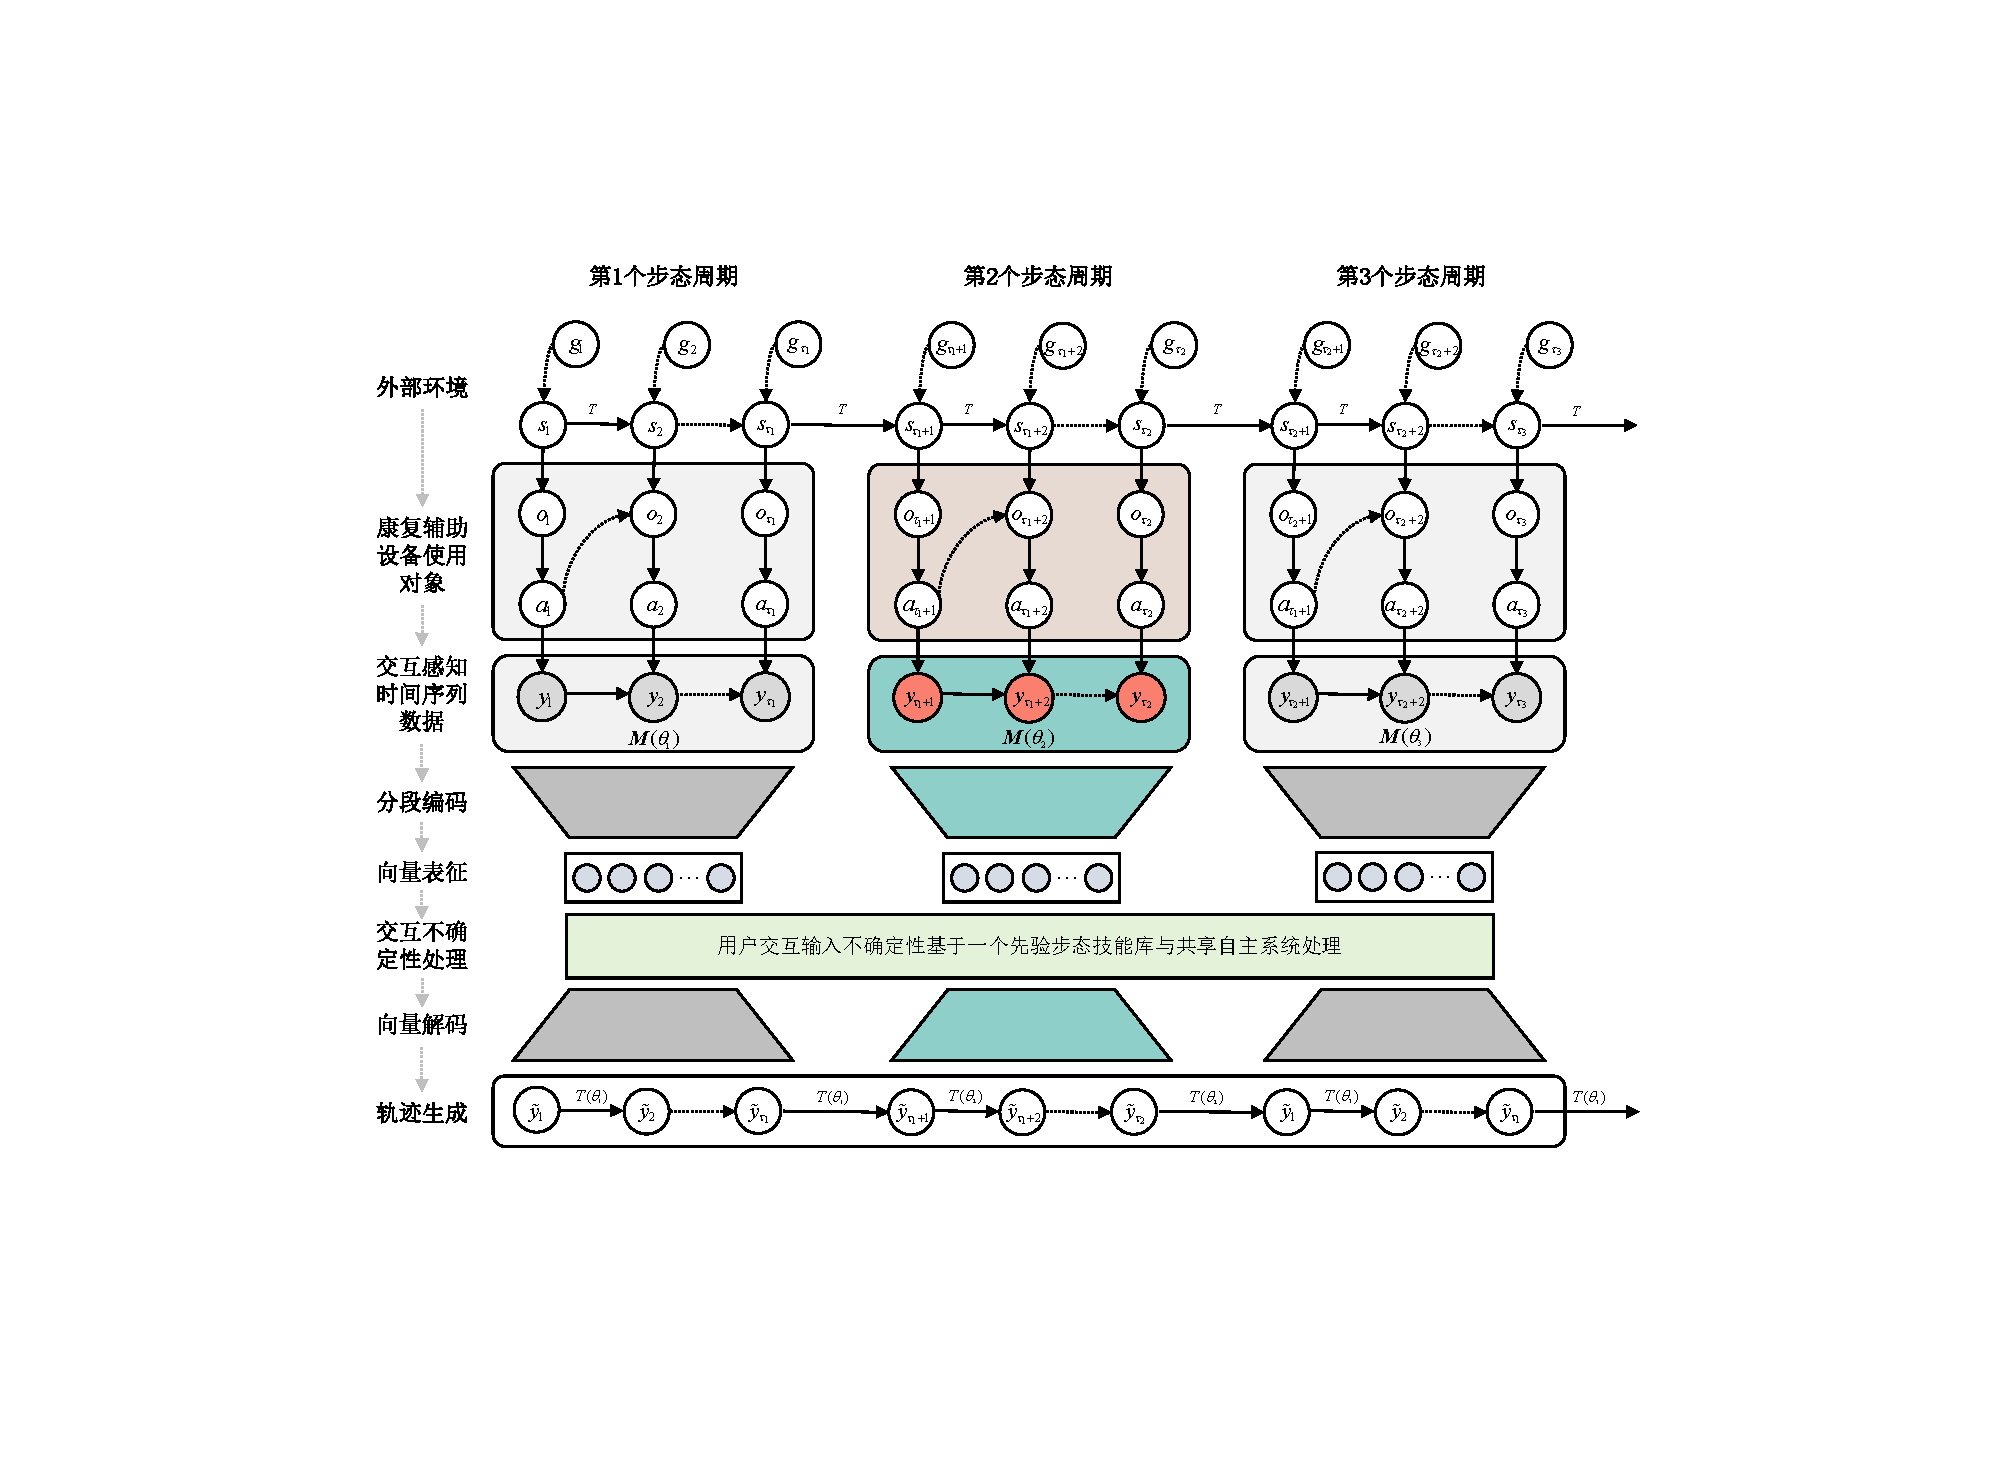
\includegraphics[width=1\textwidth]{figures/5-Fig-Intro.pdf}
  \caption{所提出交互式关节运动辅助轨迹生成算法的概率图模型}
  \label{fig:5-Intro}
\end{figure}

\section{主动式膝关节矫形器系统设计}

\subsection{主动式膝关节矫形器硬件结构}
如图\ref{fig:5-1}所示,为了验证所提出方法的效果,我们搭建了一个简化设计的主动膝关节矫形器原型样机。该样机在膝关节处安装了一个电动执行器,该执行器由配备1:100谐波减速器的Faulhaber MC5010驱动器驱动的Maxon EC90 Flat扁平直流无刷电机组成,其通过减速后产生的扭矩与膝关节周围人体肌肉提供的等效扭矩大致相当。执行器被安装在一个专用的无源碳纤维膝关节矫形器上,通过绑带固定在大腿和小腿上以辅助膝关节的运动。此外,实验中我们将膝关节矫形器通过一个自由移动的尼龙带连接至一个腰部固定装置,以将矫形器的一部分自重转移到腰部承担。在本框架中,采用了三个惯性测量单元(IMU)(Xsens DOT,Xsens Technologies)用于捕捉下肢运动。其中两个惯性测量单元分别放置于未受影响侧的大腿和小腿上,以捕获使用者自主运动时的膝关节角度;另一个惯性测量单元则放置在受影响侧的大腿上用于捕获步态相位。每个IMU单元通过低功耗蓝牙将采集得到的姿态四元数数据传输至一台搭载Intel Core i5 8500T处理器和Ubuntu 20.04操作系统的个人计算机。
\begin{figure}[htb]
  \centering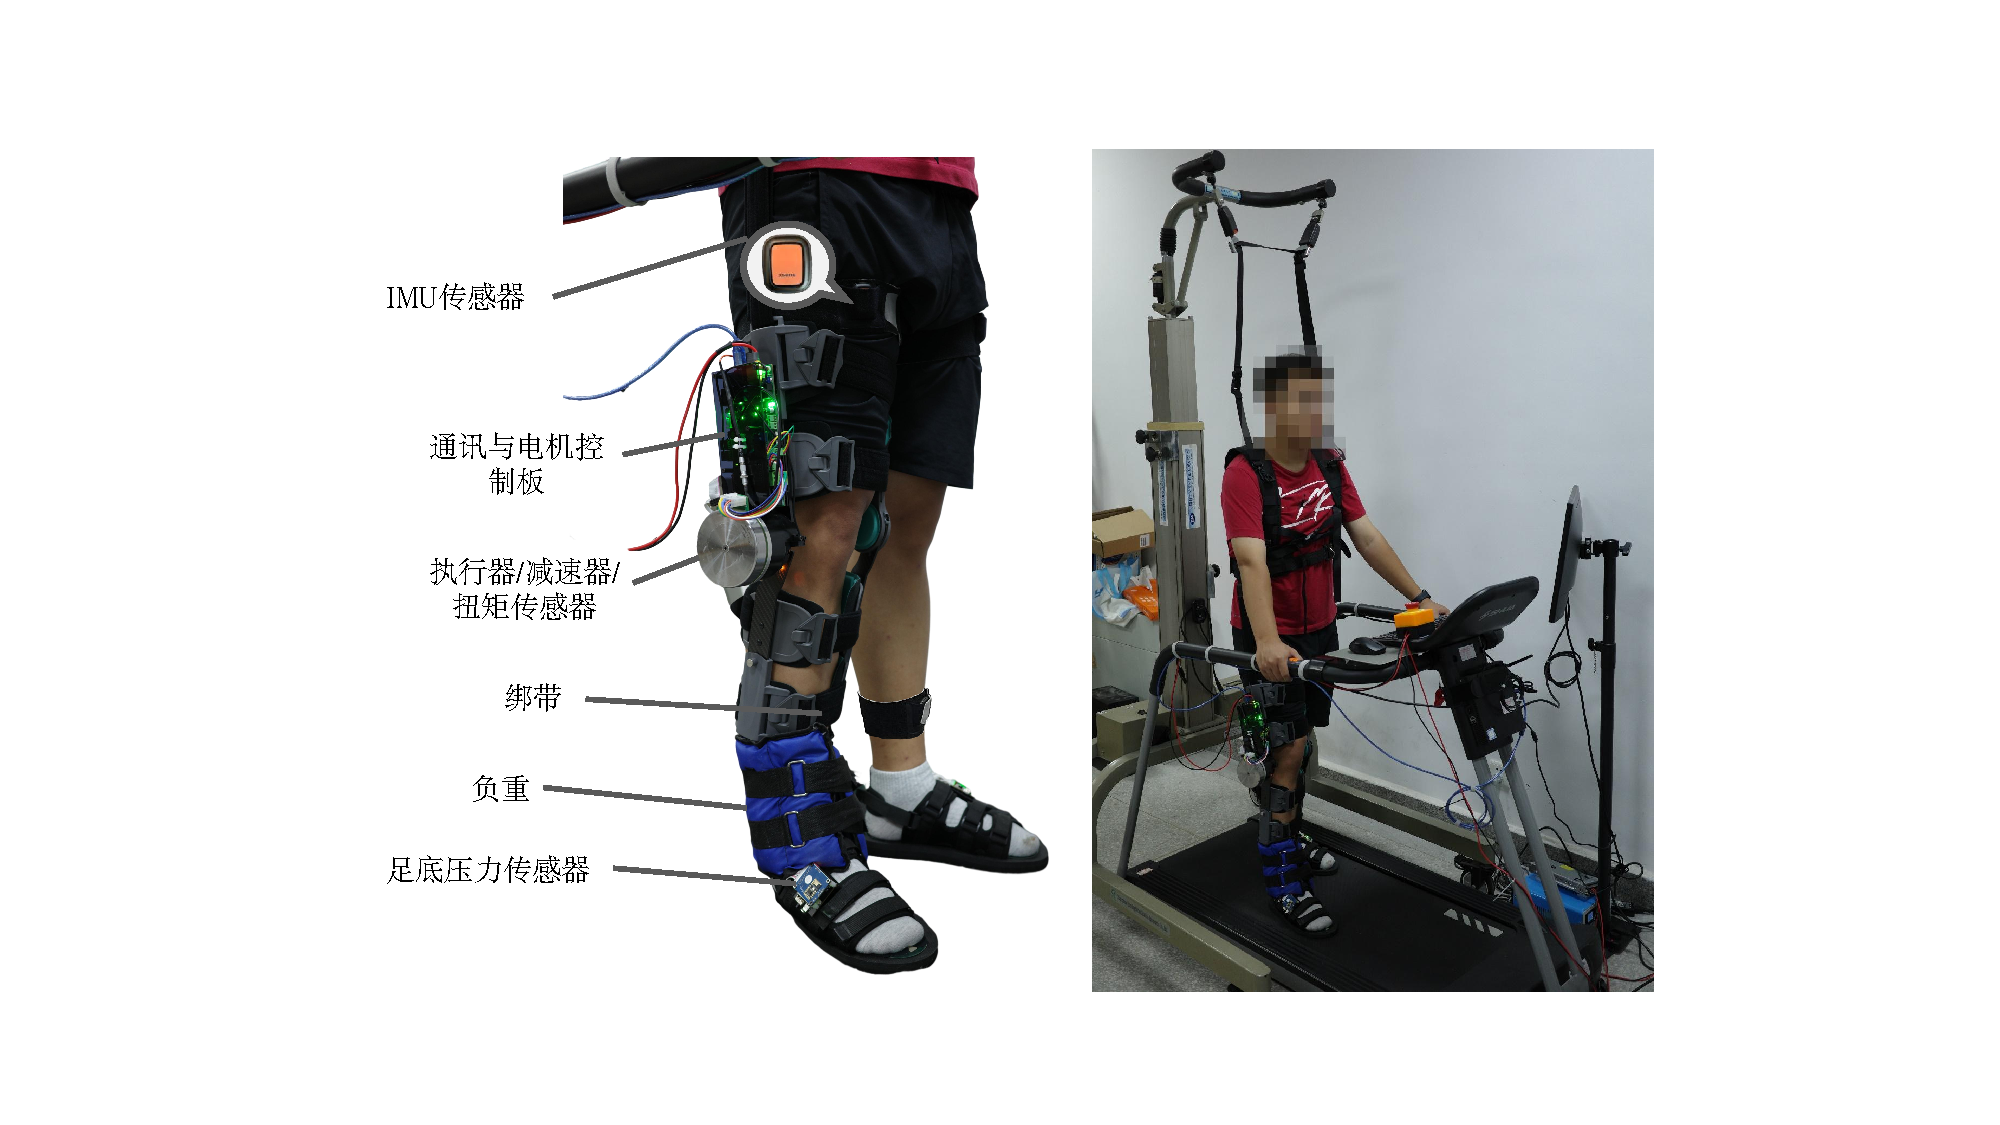
\includegraphics[width=0.9\textwidth]{figures/5-Fig-1.pdf}
  \caption{主动式膝关节矫形器硬件实物图}
  \label{fig:5-1}
\end{figure}

\subsection{轨迹生成算法框架}
所提出的算法框架基于一个编码器-解码器的结构设计,并引入了一个在线用户输入验证和仲裁机制以减少用户实时交互输入不确定性的影响。图\ref{fig:5-2}给出了该算法框架的结构示意图。其中,健侧的自主膝关节运动由位于大腿和小腿上的IMU传感器捕获,姿态数据由角度计算器计算得出膝关节的角度,并通过一个有限冲激响应(FIR)低通滤波器进行滤波(截止频率:5Hz)。为了尽可能以较低的计算负担精确捕捉实时的步态相位和步行速度,该系统基于放置在健侧和患侧大腿上的惯性测量单元与两个独立的自适应非线性频率振荡器进行耦合振荡,进而通过捕捉髋关节的运动确定可以量化的实时步态相位和步行速度。位于健侧的步态编码器负责将一个步态周期内($[0,2\pi ]$)健侧的自主膝关节运动轨迹编码到一个低维的向量空间中。步态先验技能库用于提供先验自主策略,其是通过离线采集健康受试者的步行演示数据构建而成的。共享自主系统由两个基本组件构成。第一部分为一个用户自主输入验证模块,旨在阻止任何超出GKL范围的实时用户输入传输至患侧的执行器上。第二部分为仲裁功能,用于推断用户的输入意图并将其与步态先验技能库中的策略进行动态融合。最后,将经过共享自主处理后的交互指令传输至步态解码器,并根据当前患侧的步态相位生成患侧的膝关节运动参考轨迹。

\begin{figure}[!t]
  \centering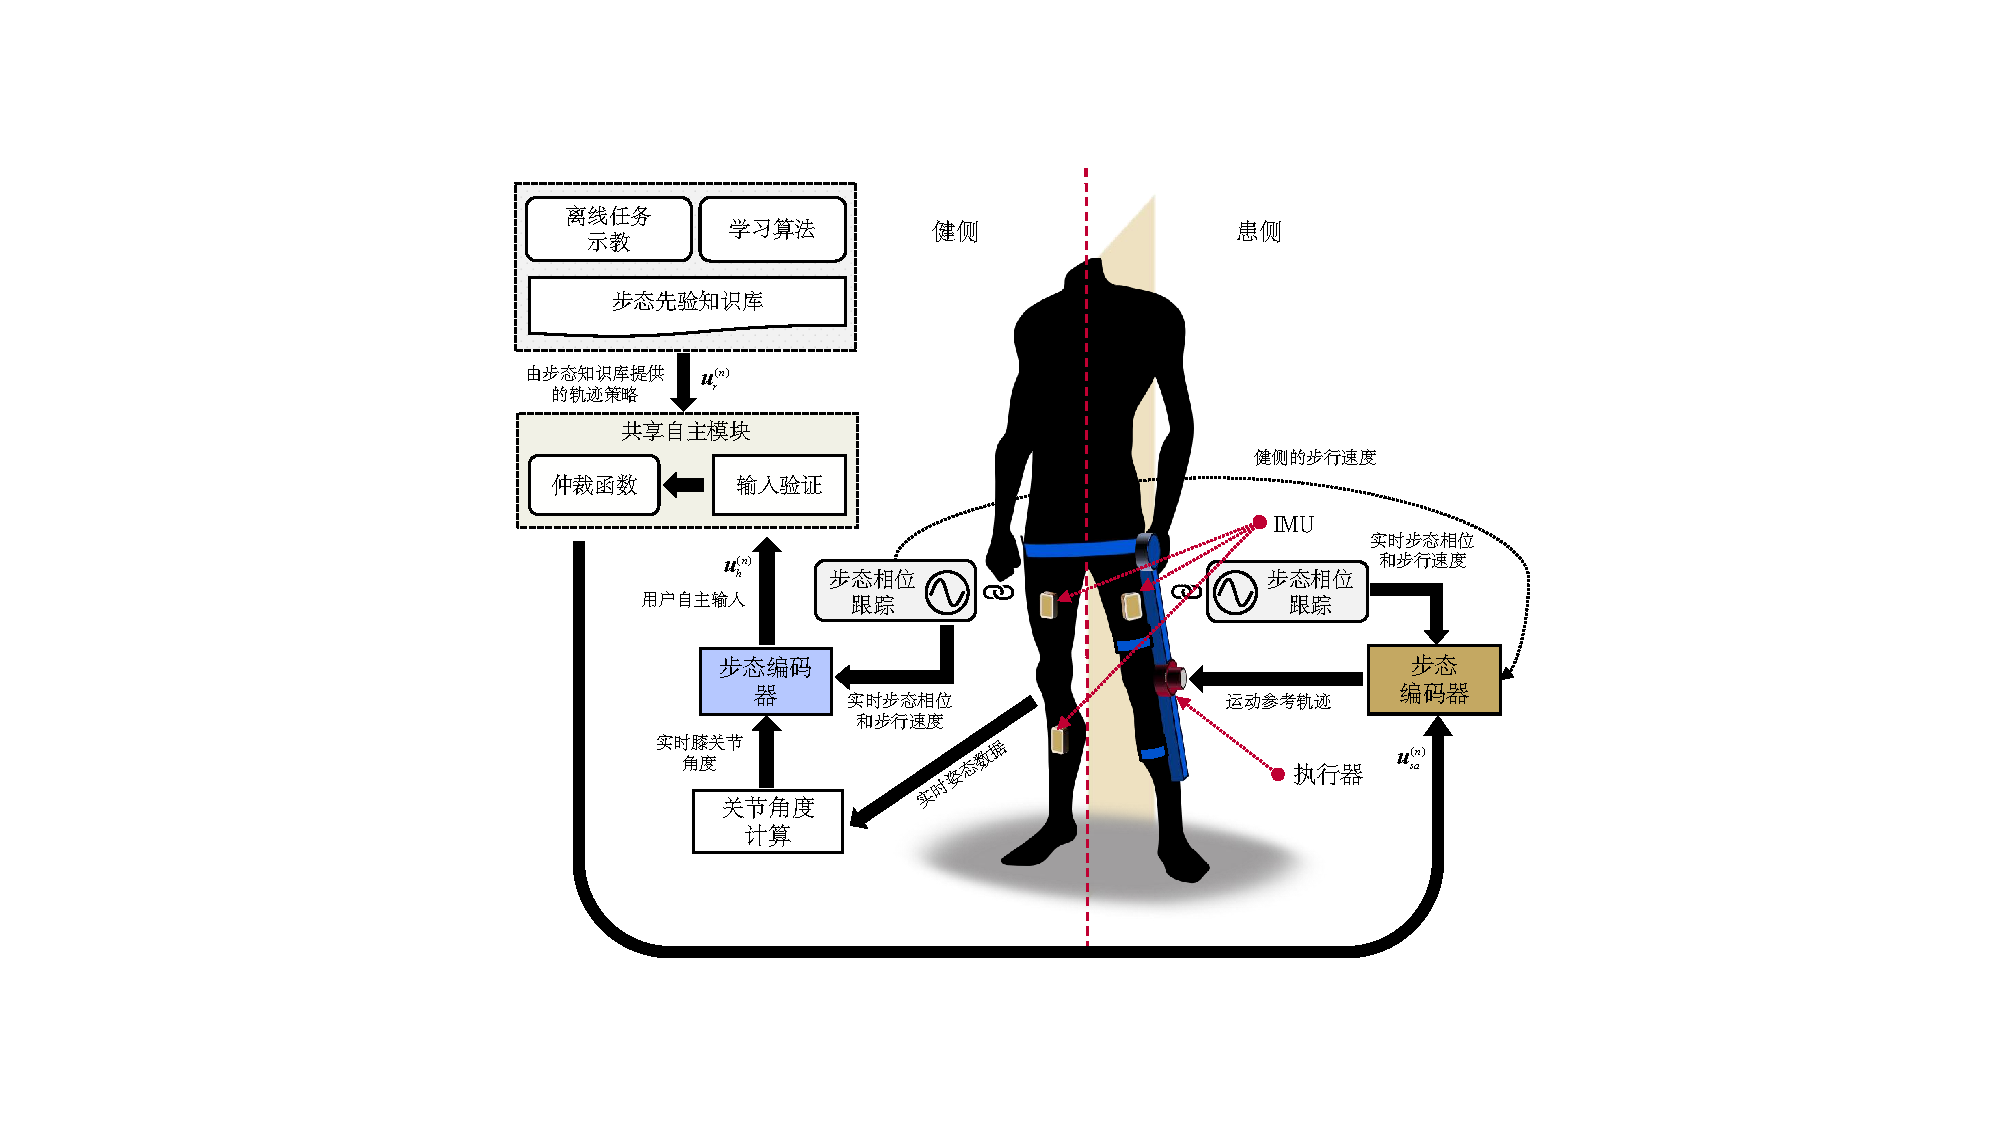
\includegraphics[width=0.8\textwidth]{figures/5-Fig-2.pdf}
  \caption{基于共享自主系统的自适应对称步态参考轨迹生成算法框架}
  \label{fig:5-2}
\end{figure}

\section{基于共享自主系统的交互式安全对称步态轨迹生成}
本节就所提出的轨迹生成算法框架进行了详细的介绍和实现。其中算法\ref{algo:5-1}给出了实现上述交互式轨迹生成框架的伪代码,并在后续小节对图中提到的变量和常量进行了定义。此外,为了清楚起见,将第$n{\rm{ - th}}$个步态周期的用户输入定义为${\pmb{u}}_h^{(n)} \in {\mathbb{R}^N}$,将共享自主模块调整后的输出定义为${\pmb{u}}_{sa}^{(n)} \in {\mathbb{R}^N}$,将由技能库提供的自主策略定义为${\pmb{u}}_r^{(k)} \in {\mathbb{R}^N}$,其中参数$k$代表了共享自主系统捕获的用户输入意图类别。
\begin{algorithm}[h]
  \SetAlgoLined
  \KwData{先验步态技能库的参数$\pmb{\mu}_k$,$\Sigma_k$}
  \KwIn{实时髋关节角度$y_{lhip}(t),y_{rhip}(t)$,实时的健侧膝关节角度$y_{lknee}(t)$}
  \KwResult{执行机构的运动参考轨迹$\widetilde{y}_{rknee}(t)$ }
  初始化自适应频率振荡器$x_1(0),x_2(0),\omega(0),\alpha_0(0)\alpha_1(0)$\;
  初始化步态编码器$w_i(0)=0$\;
  初始化用户输入$\pmb{u}_h^{(0)}=\pmb{0}$\;
  \For{$t$=1,2,3,...}
  {
    (步态相位跟踪)\\
    健侧:$\omega_l(t)$,$\phi_l(t)$=ANFO($y_{lhip}(t)$) \;
    患侧:$\omega_r(t)$,$\phi_r(t)$=ANFO($y_{rhip}(t)$) \;
    (编码健侧输入关节轨迹)\\
    \eIf{步态周期结束}
    {
      步态编码器编码轨迹:GaitEncoder($\phi_l(t),y_{lknee}(t)$) \;
    }
    {
      更新第n个步态周期的用户自主输入,并重置步态编码器:$\pmb{u}_h^{(n)}$ 
    }
    (共享自主系统)\\
    \eIf{$\omega_r(t)>Tr_\omega$和$\omega_l(t)>Tr_\omega$}
    {
      \If{用户自主输入已更新}
      {
        用户交互意图:$k=argmin(\Delta_k(\pmb{u}_h^{(n)}))$ \;
        共享自主混合输入:$\pmb{u}_{sa}^{(n)} = h_{\theta}(\pmb{u}_r^{(k)}, \pmb{u}_h^{(n)})$\;
      }
    }
    {
      停止运动:$h_{\theta}(\pmb{u}_r^{(k)}, \pmb{u}_h^{(n)})=\pmb{0}$
    }
    (解码共享自主系统输出为执行器运动参考轨迹)\\
    \eIf{步态周期结束}
    {
      更新步态解码器中的参数:$\pmb{u}_{sa}^{(n)}$,$\Omega^{(n)}$\;
    }
    {
      参考轨迹:$\widetilde{y}_{rknee}(t)$=GaitDecoder($\Delta t$, $\phi_r(t)$,$\Omega^{(n)}$,$\pmb{u}_{sa}^{(k)}$) \;
    }
  }
  \caption{自适应膝关节对称参考轨迹生成算法}
  \label{algo:5-1}
\end{algorithm}  

\subsection{步态相位跟踪} 
非线性振荡器能够模拟广泛的物理和生物过程,尤其是作为中央模式生成器(Central Pattern Generator, CPG)的数学模型。研究利用了由 Righetti 等人提出的一种具有频率自适应机制的 Hopf 振荡器 \cite{righettiDynamicHebbianLearning2006}用以与位于大腿位置的惯性传感器捕获的髋关节运动进行耦合,从而实现步态相位与步行速度的实时跟踪。Hopf振荡器的动力学由以下一组微分方程控制:
\begin{equation}
\label{deqn_ex1}
\begin{array}{*{20}{l}}
{{{\dot x}_1} = \gamma \left( {\mu  - \left( {x_1^2 + x_2^2} \right)} \right){x_1} + \omega {x_2} + \varepsilon e(t)}  \\  
{{{\dot x}_2} = \gamma \left( {\mu  - \left( {x_1^2 + x_2^2} \right)} \right){x_2} - \omega {x_1}} 
\end{array}
\end{equation}   
其中参数$\gamma= 15$决定振荡器的吸引力强度,$\varepsilon  = 0.1$是外部输入与振荡器的耦合强度,$e(t)$是外部输入的周期波动信号。如果不存在外部输入$e(t)=0$,振荡器的状态变量$[{x_1},{x_2}]$将收敛到一个幅度为$\mu=1$且振荡频率为$\omega$初始设定值的极限环上。在研究中,振荡器的实时角频率$\omega$用作表示步态速度,当以适当的耦合强度与外部输入$e(t)$的基本频率共振。自适应频率$\omega$的计算方法定义如下:
\begin{equation}
\label{deqn_ex2}
\dot \omega  = {{ - \varepsilon e(t){x_2}} \mathord{\left/
{\vphantom {{ - \varepsilon e(t){x_2}} {\sqrt {x_1^2 + x_2^2} }}} \right.
\kern-\nulldelimiterspace} {\sqrt {x_1^2 + x_2^2} }}
\end{equation}    

其中健侧和患侧的步态速度分别定义为${\omega _l}(t)$和${\omega _r}(t)$。为了加快耦合振荡器的收敛速度并增强其稳定性,如式\ref{deqn_ex3}所示,对由惯性传感器捕获的髋部运动${y_{hip}}(t)$进行了负反馈处理。其中$\hat y(t)$是ANFO的反馈项,式\ref{deqn_ex3}中的求和项是一个滑动窗口平均因子,用于消除窗口长度为$T = 50$内的髋部运动基准偏移。
\begin{equation}
\label{deqn_ex3}
e(t) = {y_{hip}}(t) - \frac{1}{T}\sum\limits_{i = t - T + 1}^t {{y_{hip}}(i)}  - \hat y(t)
\end{equation}   

\begin{equation}
\label{deqn_ex4}
\hat y(t) = {\alpha _0}(t) + {\alpha _1}(t){x_1}(t)
\end{equation}    
其中动态变化的系数${\alpha _0}(t)$和${\alpha _1}(t)$的定义如下:
\begin{equation}
\label{deqn_ex5}
{\dot \alpha _0}(t) = \eta e(t)
\end{equation}   
\begin{equation}
\label{deqn_ex6}
{\dot \alpha _1}(t) = \eta e(t){x_1}(t)
\end{equation} 
积分增益设置为$\eta=2$,振荡器的动态系统初始值设置为$[{x_1},{x_2},\omega ,{\alpha _0},{\alpha _1}] = [1,0,1,0,0]$。瞬时步态相位$\phi (t)$可以通过以下方式计算:
\begin{equation}
\label{deqn_ex7}
\phi (t) = \arctan 2({x_2}(t),{x_1}(t)) + \pi 
\end{equation}    
由于在该框架中需要对每个步态周期来自健侧的运动轨迹进行编码表征,并作为用户自主输入送入共享自主系统,因此需要对每个步态周期进行在线的分割。利用自适应振荡器的相位突变点可以用很低的成本实现这一目标,当两个时间步之间的相位差$\lvert \phi (t) - \phi (t - 1) \rvert \geq 6$时,则发生一次相位突变事件,并在此处为一个步态轨迹分割位置实现对步态时间序列的分段处理。  

\subsection{步态行为表征与编码} 步态编码器通过在线学习,将不定长度且连续时间的膝关节步态运动轨迹压缩为固定长度的向量。选用适当的人类行为表征方式是构建共享自主系统的基础,这涉及如何对行为进行建模以及如何有效地执行验证和纠正。这包括捕捉行为的复杂性、不确定性和多样性,以便系统能够在各种情况下准确识别用户的意图并进行适当的调整。同时,验证和纠正机制也是确保系统稳定运行的关键环节,它们有助于过滤掉不安全的输入,并确保系统始终遵循预定的策略。因此,在设计共享自主系统时,需要综合考虑人类行为的特点,以及如何将这些特点融入系统的验证和纠正机制中。在本研究章节中,我们借助模仿学习算法\cite{schaalImitationLearningRoute1999}将膝关节角度的时间序列数据映射至低维子空间,以实现对其的适当调整。考虑到步行运动是典型的周期性行为,采用第二章所述的节律型动态运动基元(pDMP)\cite{ijspeertDynamicalMovementPrimitives2013,gamsOnlineLearningModulation2009}对步态行为编码表征到实时相位空间当中。然而,倘若容许时间尺度项发生动态变化,则优化过程或许会陷入不稳定状态。因此,在本实现方案中固定了pDMP中的周期调制参数$\Omega  = 1$,以确保优化过程的稳定性。通过重写pDMP可以获得学习目标${f_{targ}}(t)$为:
\begin{equation}
  {f_{targ}}(t) = {\ddot y_{knee}}(t) - {\alpha}({\beta}( - {y_{knee}}(t)) - {\dot y_{knee}}(t))
  \label{eq:5-1}
\end{equation}    

其中${\dot y_{knee}}(t)$、${\ddot y_{knee}}(t)$是健侧膝关节的运动角度轨迹${y_{knee}}(t)$的一阶和二阶导数。优化损失函数${J_i}$定义为:
\begin{equation}
  \label{deqn_ex12}
  \begin{array}{*{20}{c}}
    {{J_i} = \sum\limits_{t = 1}^P {{\psi _i}} (t){{\left( {{f_{targ}}(t) - {w_i}r} \right)}^2}}&{,i = 1,2,...,N} 
  \end{array}
\end{equation}       

其中在本研究中$N=20$表示将一个步态周期中膝关节运动轨迹编码后权重向量长度,损失函数${J_i}$的最小化可以通过一个递归最小二乘法(RLS)来在线实现,其可以通过迭代优化学习pDMP中的局部线性模型的权重向量$\pmb{w}(t)=({w_1}(t),{w_2}(t),...,{w_N}(t))$实现。当在时间$t$捕获到一个步态相位突变事件时表明完成了一个完整的步态周期运动,此时根据步态编码器的输出,定义用户输入为$\pmb{u}_r^{(n)} = \pmb{w}(t)$。令$\pmb{u}_r^{(n)} = (w_1^{(n)},w_2^{(n)},...,w_N^{(n)})$为第$n{\text{ - th}}$个步态周期的用户输入,$\pmb{u}_r^{(n + 1)} = (w_1^{(n + 1)},w_2^{(n + 1)},...,w_N^{(n + 1)})$为下一个步态周期用户输入。由于膝关节的运动轨迹在分割点之前和之后保持一致的模式,因此可以两个编码后的用户输入在解码后实现每个连续用户步态输入的无缝转换衔接(其中$w_N^{(n)}\approx w_1^{(n+1)}$)。在每个步态周期完成后,将触发一个步态周期分割事件。此时,用户输入将被发送至共享自主系统,以便对该输入的合理性进行判断和仲裁。完成传输后,用户的自主输入矢量$\pmb{w}(t)$随后重置为其初始状态。

\subsection{步态技能库}研究设置的包含两种动作参数组的步态技能库$\mathscr{L}=\left\{\Theta^{walking},\Theta^{upstair}\right\}$是通过对健康受试者进行离线演示以及步态编码器收集的数据构建而成。在这部分研究中,我们假定具有相同运动模式$ k $的步态运动轨迹的权重向量是相互独立的。其中参数组$\Theta^k \sim {\mathcal{N}}\pmb{(}{{\pmb{\mu }}_k},{\Sigma _k}\pmb{)}$服从多维高斯分布。期望${{\pmb{\mu }}_k} \in {\mathbb{R}^N}$和协方差矩阵${\Sigma _k} \in {\mathbb{R}^{N \times N}}$可以通过最大似然估计从演示数据中进行计算获得。在此基础上,由步态技能库提供的策略从技能库中采样得到,可定义如下:$\pmb{u}_r^{(k)}\leftarrow \Theta$。

\subsection{防止不确定交互输入的共享自主系统设计}
\subsubsection{自主输入验证}鉴于用户输入的不确定性和多变性,其验证和筛选显得尤其关键。在动态运动基元的核心特性中,相似轨迹的拓扑结构会导致相应在pDMP中的权重向量显示出相似性。也就是说,通过比较由pDMP编码的不同交互输入权重向量,可以评估输入之间的相似程度,以实现对用户输入的有效验证和筛选\cite{ijspeertDynamicalMovementPrimitives2013}。该问题可以视为一个在线异常检测问题,因此在输入验证模块中,研究采用了基于距离度量的奇异输入检测方法。相较于其他方法,这种方法具有形式简单、计算量较低的优势。具体而言,步态轨迹输入的相似度距离度量定义如下:
\begin{equation}
  \label{deqn_ex13}
  {\Delta _k}({\pmb{u}}_h^{(n)}) = \sqrt {{{({\pmb{u}}_h^{(n)} - {{\pmb{\mu }}_k})}^T}\Sigma _k^ - ({\pmb{u}}_h^{(n)} - {{\pmb{\mu }}_k})} 
\end{equation}   

\begin{equation}
  \label{deqn_ex14}
  k = \arg \min \left( {{\Delta _k}({\pmb{u}}_h^{(n)})} \right)
\end{equation}
其中${\Delta _k}(\pmb{u}_h^{(n)})$是来自用户健侧的步态轨迹编码输入${\pmb{u}}_h^{(n)}$与步态技能库中策略之间的马氏距离。马哈拉诺比斯距离是由印度统计学家马哈拉诺比斯提出的,用于计算数据中的协方差距离。这种距离衡量方法可以有效地计算两个未知样本集合的相似度。与欧式距离不同,马哈拉诺比斯距离考虑了各个特征之间的相关性(例如,身高信息可能与体重信息相关),并且具有尺度不变性,即它不受测量尺度的影响。下标$k$表示用户意图执行的步态模式,其通过最小距离准则在线动态确定。但是,由于节律型DMP的特殊结构,其编码后局部线性模型的权重向量的第一项始终等于向量中的最后一项${w_1}(t)={w_N}(t)$。这导致在协方差矩阵${\Sigma _k}$中存在线性相关的行向量,因此无法直接计算其逆矩阵。为了解决这一问题,在公式\ref{deqn_ex13}中,$\Sigma_k^-$是广义逆矩阵,它将多维高斯分布退化到一个较低维子空间,但不影响距离测量。最终,当距离度量超过设定的阈值时,系统认为该自主输入是奇异的${\Delta _k}(\pmb{u}_h^{(n)}) > T{r_k}$。  

\subsubsection{仲裁函数}仲裁函数在构建共享自主系统中具有至关重要的作用,其核心在于根据用户输入意图的置信度进行实时在线微调。为实现这一目标,所提出方法采用步态技能库中的先验策略与用户的自主输入进行在线调整的线性组合。这种方法在保持轨迹个性化的基础上,有效降低了动态变化环境中人机交互输入的不确定性影响,从而确保了康复机器人运动规划的安全性和可靠性。围绕这一问题,本章研究中的共享自主模块采用了一个具有时变混合系数的仲裁函数进行参数化。这一设计旨在实现在用户输入与步态技能库所提供的策略之间进行无缝切换。混合命令定义为${\pmb{u}}_{sa}^{(n)} = {h_\theta }({\pmb{u}}_r^{(k)},{\pmb{u}}_h^{(n)})$,该仲裁函数定义如下:
\begin{equation}
  \label{deqn_ex15}
  {h _\theta } \triangleq \left \{  {\begin{array}{*{20}{c}}
    {\pmb{\lambda }_\theta ^{(n)}{\pmb{u}}_h^{(n)} + \left( {1 - {\boldsymbol{\lambda }}_\theta ^{(n)}} \right){\pmb{u}}_r^{(k)}}&{{\text{, gait speed }}\pmb{ >  }T{r_\omega }}  \\  
    \pmb{0}&{{\text{, gait speed }}\pmb{ <  }T{r_\omega }} 
  \end{array}} \right.
\end{equation}

其中混合系数是一个和步态编码器输出维度相同的权重向量组成的${\pmb{\lambda }}_\theta ^{(n)} = [\lambda _1^{(n)},\lambda _2^{(n)},...,\lambda _N^{(n)}]$,向量元素$\lambda _{1,2,...,N}^{(n)} \in [0,1]$。该系数向量通过在步态技能库中实时在线地调整用户输入与策略之间的控制权限分配,从而实现动态自主性。这一方法使得共享自主系统能够灵活应对环境的变化,同时保持用户输入的个性化特征,进而提高康复机器人运动规划的适应性与安全性。当$\lambda _{1,2,...,N}^{(n)} = 0$表示规划出的运动参考轨迹完全依赖于步态技能库中提供的先验预定义策略时。相反,当$\lambda _{1,2,...,N}^{(n)} = 1$时,患侧驱动器的运动参考轨迹完全基于用户的自主输入。与输入验证模块不同,仲裁功能主要在轨迹细节层面纠正用户输入${\pmb{u}}_h^{(n)}$中严重偏离步态技能库中先验知识的元素。混合系数${\pmb{\lambda }}_\theta ^{(n)}$代表在系统对用户自主输入的信心,其由一个非线性函数计算得出:
\begin{equation}
  \label{deqn_ex16}
  {\pmb{\lambda }}_\theta ^{(n)} \triangleq {\text{exp}}\left( {{\text{ - }}{{{\pmb{d}^{(n)}}} \mathord{\left/
 {\vphantom {{{\pmb{d}^{(n)}}} \theta }} \right.
 \kern-\nulldelimiterspace} \theta }} \right)
\end{equation} 

\begin{equation}
  \label{deqn_ex17}
  {\pmb{d}^{(n)}} = {\left[ {diag({{\Sigma _k}})} \right]^{ - 1}} \cdot \left( {\pmb{u}_h^{(n)} - {\pmb{\mu }_k}} \right) \odot \left( {\pmb{u}_h^{(n)} - {\pmb{\mu }_k}} \right)
\end{equation}

其中相似性度量${\pmb{d}^{(n)}} \in {\mathbb{R}^N}$是通过将用户输入与步态技能库中的策略进行比较而获得的标准化距离。超参数$\theta>0$用于调整在相同的距离偏移度量下的人机信任级别,其可以根据经验设置或通过基于在线人机循环的算法动态优化。当$\theta \to \infty$时,仲裁函数对用户的自主输入变得更加敏感(允许用户输入与技能库中的先验信息之间存在更大的偏移),当$\theta \to 0$时,混合命令${\pmb{u}}_{sa}^{(n)}$将主要受技能库中预定义的策略的支配。

除能使自适应频率振荡器收敛至极限环的稳定周期性步态模式外,本研究还探讨了两种需单独处理的非周期性过渡状态。其中,``开始''事件指的是从初始状态(各关节角度为零)进入稳定的周期性步态;而``停止''事件则是指从稳定的周期性步态恢复到初始状态。为处理这两种非周期性过渡状态,所设计系统采用了相应的两种策略,以确保康复机器人在运动过程中的连贯性与稳定性。其中 ``开始''事件触发后由引导动作${\pmb{u}^{(start)}} = ({u}_1^{(start)},{u}_2^{(start)},...,{u}_N^{(start)})$进行处理,当用户输入首次通过输入验证模块时,该操作用于将轨迹目标从初始状态平滑地过渡到周期性步态模式。
\begin{equation}
  \label{deqn_ex18}
  \begin{array}{*{20}{c}}
    {{u}_i^{(start)} \triangleq \frac{N}{{N - 1}}\left( {1 - \frac{{w_N^{(start)} - 1}}{{i - N-1}} + \frac{{w_N^{(start)}}}{N}} \right)} 
  \end{array}
\end{equation} 
其中$w_N^{(start)}$是第一个有效的用户自主输入向量中的最后一项。当健侧或患侧的步态速度低于某个阈值$T{r_\omega }$时,“停止”事件将被触发,其表明用户意图停止步态训练,并将规划轨迹引导至初始状态。

\subsection{步态轨迹解码}步态解码器可以被认为是一个时变线性系统,将pDMP使用欧拉法离散化后。考虑到健侧与患侧的自适应频率振荡器(ANFO)是相互独立运行的,因此其能够直接生成自适应步态相位延迟,而无需保存运动数据。步态解码器所生成的参考轨迹${{\tilde y}_{rknee}}(t)$定义为:
\begin{equation}
  \label{deqn_ex19}
  \pmb{s}(t) = {{\mathbf{A}}^{(n)}}\pmb{s}(t - 1) + {\mathbf{B}}\pmb{u}(t)
\end{equation}

\begin{equation}
  \label{deqn_ex20}
  {{\tilde y}_{rknee}}(t) = {\mathbf{C}}\pmb{s}(t)
\end{equation}    
状态向量$\pmb{s}(t)={\left[ {z(t),y(t)} \right]^T}$和${\pmb{u}}(t)=r \cdot f({\phi _r}(t),{\pmb{u}}_{sa}^{(n)})$,矩阵${\mathbf{B}={\left[ {\begin{array}{*{20}{c}}1&0 \end{array}} \right]^T}}$和${\mathbf{C}=\left[{\begin{array}{*{20}{c}}0&1 \end{array}} \right]}$。时变转移矩阵${{\mathbf{A}}^{(n)}}$定义为:

\[{{\mathbf{A}}^{(n)}} = \left[ {\begin{array}{*{20}{c}}
{ - {\Omega ^{(n)}}{\alpha}\Delta t}&{ - {\Omega ^{(n)}}{\alpha}{\beta}\Delta t}  \\  
{{\Omega ^{(n)}}\Delta t}&0 
\end{array}} \right]\]    
其中$\Delta t$是积分时间步长,${\Omega ^{(n)}} = {{\omega _r^{(n)}} \mathord{\left/{\vphantom {{\omega _r^{(n)}} {\omega _l^{(n)}}}} \right.\kern-\nulldelimiterspace} {\omega _l^{(n)}}}$。

\section{实验与分析}本节评估了所提出的基于惯性运动捕捉数据的框架在各种人机信任超参数设置及多任务场景下的性能表现。此外,研究还利用开发的主动式膝关节矫形器原型,在实际场景中对辅助行走框架的有效性进行了实证检验。9名健康受试者(年龄$26\pm 4$;性别:男;身高:$175\pm 14$cm;体重:$66\pm13$kg)参与了本实验研究并签署了知情同意书。在每次实验之前,将惯性传感器单元及其附属肢体之间的姿态关系校准到初始状态\cite{tongLSTMBasedLowerLimbs2020}。其中两名受试者的数据用于构建步态技能库,七名受试者的数据用于测试。  

所设计主动式膝关节矫形器样机采用了一种带有前馈重力补偿的比例-微分(PD)控制器用于控制执行器,使其能够准确地跟踪所提出方法生成的步态参考轨迹。相关研究\cite{zanottoAdaptiveAssistasneededController2014a}表明,在下肢施加超过2千克的负载可以显著改变步态运动学,从而模拟偏瘫步态。为评估所提出框架在辅助步行方面的效能,实验在健康受试者的右脚踝部位附加了一个3公斤重的沙袋,以此模拟偏瘫患者的患侧步态特征。同时,在受试者脚背上方安置了两个额外的惯性测量单元(IMU),以便根据预设规则对步态的摆动阶段与站立阶段加以区分。这一实验设计旨在全面考察所提框架在不同条件下的性能表现。

% \begin{figure}[!t]
%     \centering
%     \includegraphics[width=2.6in]{figures_pdf/figures_2}
%     \caption{开发的AKO原型机及其用于辅助步行实验的控制策略。  }
%     \label{fig_2}
% \end{figure}     

\subsection{实验评估与分析指标}步态对称性的描述主要可以从时间对称性和空间对称性两个方面进行探讨。在时间对称性方面,主要关注步态周期中左右腿的运动是否具有相等的时间特性;而在空间对称性方面,则关注左右腿在空间中的运动轨迹是否具有相似性或一致性。步态时间对称性常用的量化方法是罗宾逊指数\cite{viteckovaGaitSymmetryMeasures2018},也称为对称指数(SI),其计算公式为:
\begin{equation}
\label{deqn_ex21}
{SI}{\text{ = }}\left[ {{{2 \cdot \left( {{X_l} - {X_r}} \right)} \mathord{\left/
{\vphantom {{2 \cdot \left( {{X_l} - {X_r}} \right)} {\left( {{X_l} + {X_r}} \right)}}} \right.
\kern-\nulldelimiterspace} {\left( {{X_l} + {X_r}} \right)}}} \right] \times 100 \%  
\end{equation}

其中${X_{\text{l}}}$和${X_r}$是健侧和患侧的步态支撑相时间。$SI$越接近零,则表明步态的时间对称性越好。此外,使用下肢两侧膝关节运动轨迹的时间序列${y_l(t)}$和${y_r(t)}$之间的相关系数 (CC)\cite{gouwandaIdentifyingGaitAsymmetry2011}来评估关节运动学的空间对称性。
\begin{equation}
\label{deqn_ex22}
CC = {{\sum\limits_{i = 1}^T {\left( {{y_l}(i - \tau) - {{\bar y}_l}} \right)} \left( {{y_r}(i ) - {{\bar y}_r}} \right)} \mathord{\left/
{\vphantom {{\sum\limits_{i = 1}^T {\left( {{y_l}(i) - {{\bar y}_l}} \right)}\left( {{y_r}(i + \tau ) - {{\bar y}_r}} \right)} {{\sigma _l}{\sigma _r}}}} \right.
\kern-\nulldelimiterspace} {{\sigma _l}{\sigma _r}}}
\end{equation}
其中$\tau$是两个系列之间的相位延迟,可以由自适应频率振荡器生成,${\sigma _l}$和${\sigma _r}$是方差,$\bar y_l$和$\bar y_r$是${T}$时间步内的平均值。尽管仅依赖这两个指标尚无法实现对物理人机交互系统的全面评估(因为它们并未涵盖与用户密切相关的指标,如舒适度、独立性或满意度等),但这些指标仍可在一定程度上为本章所提出的方法提供定量的评价依据。通过结合这些指标以及其他相关因素,可以更全面地了解所提出方法在实际应用中的表现。

\subsection{步态技能库的建立}步态技能库是根据两名健康受试者的动作捕捉数据建立的。受试者被要求完成两项任务(``行走''任务:在跑步机上以 0.5km/h 的稳定速度行走 3 分钟;``上楼梯''任务:以舒适的速度爬上 4m 高的楼梯并重复五次)。步态编码器负责将收集到的运动数据编码为权重向量,并通过人工方式剔除异常数据。经过这一处理过程,我们最终成功获取了136个有效的``行走''步态周期以及115个``上楼梯''步态周期数据。图\ref{fig:5-3}显示了两种步态模式下步态技能库中的权重向量各元素的分布情况。对步态技能库的分量进行 Shapiro-Wilk (SW) 正态性检验,结果表明它们与高斯分布($p<0.05$)没有显著差异,符合假设。
\begin{figure}[htb]
  \centering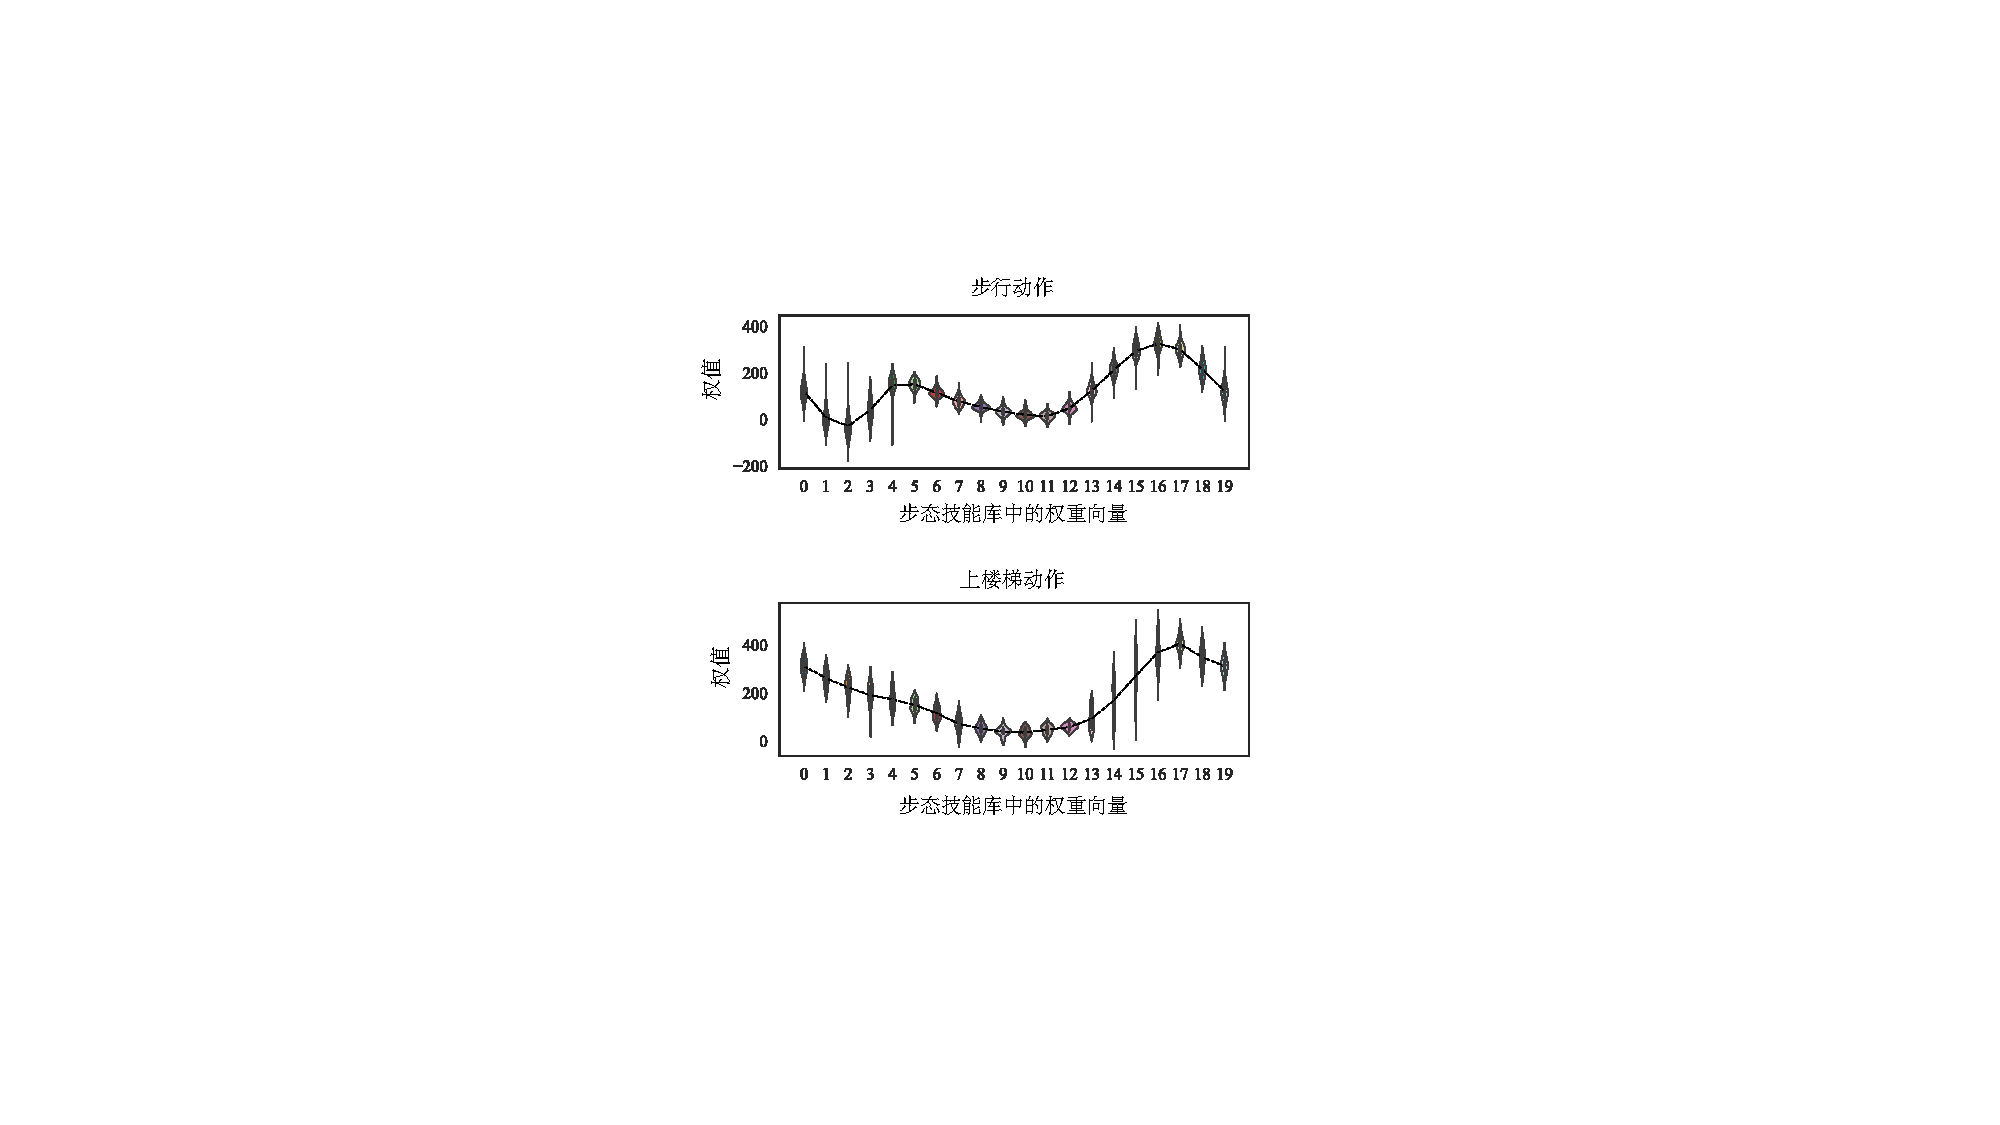
\includegraphics[width=0.7\textwidth]{figures/5-Fig-3.pdf}
  \caption{步态技能库中权重向量各元素的分布情况}
  \label{fig:5-3}
\end{figure}

\subsection{在不同人机信任参数下的轨迹生成}
为了评估所提出的轨迹生成算法框架在不同信任参数$\theta $设置下的特性,实验利用了一名健康受试者在``行走''任务中,在不佩戴主动式膝关节矫形器的情况下的健侧和患侧的运动数据进行评估。为清晰表述,此处保留了术语``健侧''和``患侧'',并将生成的轨迹与未受影响侧的用户输入数据以及受影响侧的实际膝关节轨迹进行了对比分析。这一实证研究有助于深入了解所提出方法在不同条件下的表现,并为进一步优化和完善算法提供有价值的参考。图\ref{fig:5-4}显示了当步态技能库中用户输入和先验策略之间的马氏距离增加时,在不同人机信任参数$\theta $设置下混合系数$\pmb{\lambda }_\theta ^{(n)}$随着马氏距离增加的变化曲线。

\begin{figure}[htb]
  \centering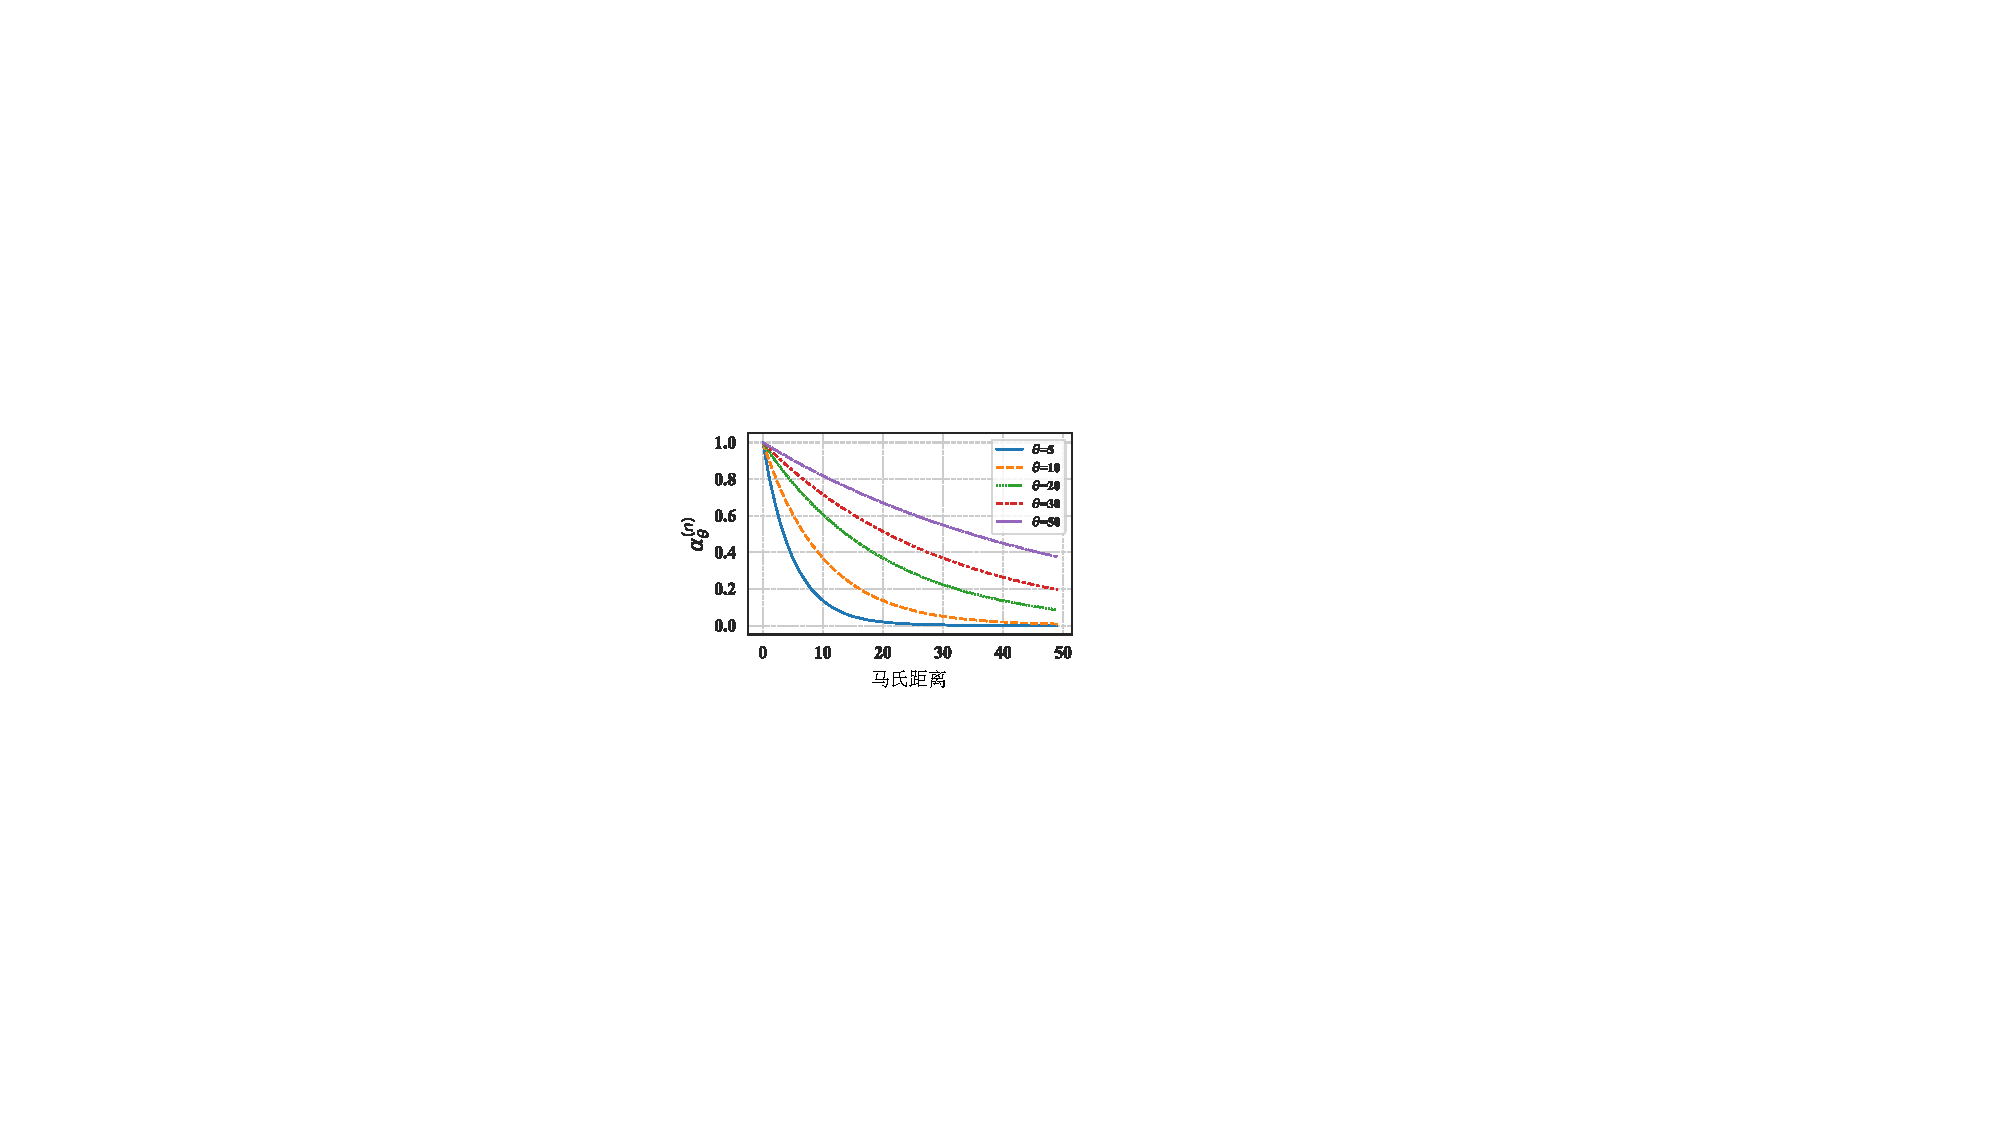
\includegraphics[width=0.5\textwidth]{figures/5-Fig-4.pdf}
  \caption{人机信任系数$\theta $从5变化到50的过程中的共享自主混合系数$\pmb{\lambda}_\theta ^{(n)}$形状}
  \label{fig:5-4}
\end{figure}

图\ref{fig:5-5}给出了在``行走''任务中的两个不同的健侧和患侧的步态轨迹。第一个代表正常的用户输入,而第二个则展示含有明显噪声的交互输入。所有五个$\theta$设置在第一个步态周期中都显示出具有良好空间对称性($CC<0.95$)的近似性能。相反,由于用户输入和步态技能库中的先验策略之间的偏差很大,共享自主系统在第二个步态周期中对用户的输入进行了矫正。实验结果如表\uppercase \expandafter{\romannumeral1}所示,其中${CC}({y_{lknee}},{\tilde y_{rknee}})$由健侧和患侧膝关节数据计算得出,${CC}({y_{rknee}},{\tilde y_{rknee}})$由患侧数据和真实数据计算得出。随着$\theta $的增加,它们呈现出相反的趋势,这是由于共享自主系统在相同条件下更加信任来自用户的自主输入造成的。然而,部分研究表明,一定程度的步态不对称可能实际上是对中风相关神经缺陷的积极适应。这表明在步态康复过程中,过于追求完美的步态对称性可能并非最佳策略。相反,应关注个体差异和患者的具体需求,以实现功能恢复和生活质量的提升\cite{balabanGaitDisturbancesPatients2014}。为了优化超参数$\theta $,可能需要进一步整合接触力或耗氧量等信息。然而,在本章的工作中,我们并未将追求高相关性作为最终目标,而是采用了经验值来设定$\theta $。这种方法有助于简化问题复杂性,同时仍能展现出所提出方法在步态康复中的潜在价值。未来研究可以在此基础上,进一步探索如何利用更多的生物力学信息来优化超参数设置,从而提高方法的性能和临床适用性。作为一种权衡选择,在后续的实验中均保持了$\theta =20$。


\begin{figure}[htb]
  \centering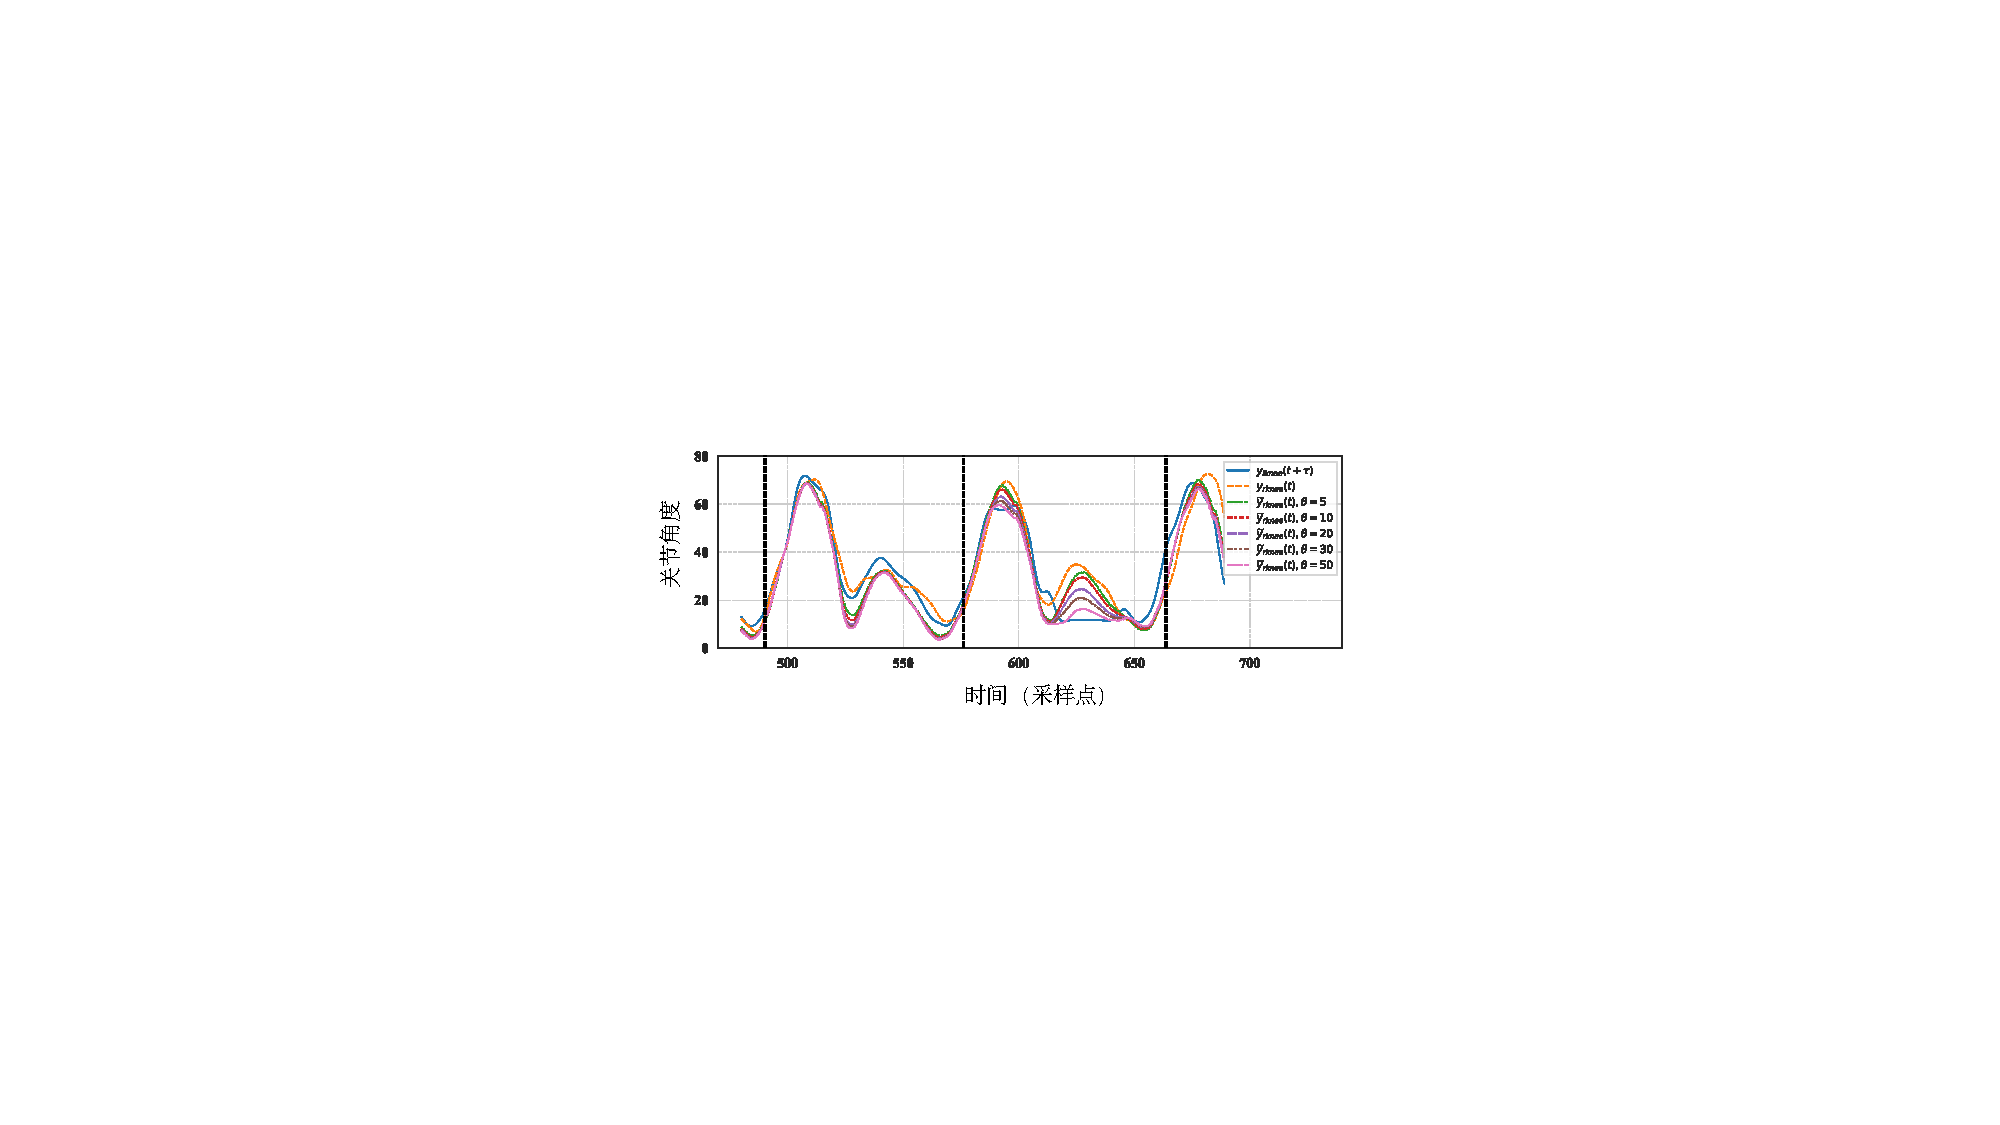
\includegraphics[width=0.8\textwidth]{figures/5-Fig-5.pdf}
  \caption{在不同$\theta $设置的具有干扰的用户自主输入下,所提出算法框架生成的参考轨迹,其中${y_{lknee}}(t - \tau )$是未受影响侧移动步态周期$\tau $个长度的关节角度,${y_{rknee}}(t)$是受影响侧的真实关节角度。}
  \label{fig:5-5}
\end{figure}

\begin{table}[htb]
  \centering
  \caption{不同$\theta $设置下的步态空间对称性指标}
  \begin{tabular}{cccccc}
  \toprule
          $\theta $         & 5 & 10 & 20 & 30 & 50  \\ 
  \midrule
          ${CC}({y_{lknee}},{\tilde y_{rknee}})$         & 0.86	&0.89	&0.93	&0.95	&0.97  \\ 
          ${CC}({y_{rknee}},{\tilde y_{rknee}})$         & 0.98 &0.97	&0.94	&0.92	&0.89  \\ 
  \bottomrule
  \end{tabular}
  \label{tab:5-1} 
\end{table}   

\subsection{不同任务下的轨迹生成}为全面评估所提出框架的性能,在实验中进一步设计了一系列涵盖多个任务的连续运动,包括行走、停止与上楼梯。这些动作由七名受试者执行,其中一名受试者的数据如图\ref{fig:5-6}所示。实验结果表明,该算法框架需约$4\pm 1$个步态周期(平均 8.6 秒)的适应周期(图\ref{fig:5-6}中的蓝色标记区域)。在此期间,共享自主模块无法确定用户的真实交互意图${k}$,因为自主输入关于两种步态动作的相似度距离度量${\Delta _k}(\pmb{u}_h^{(n)})$均大于阈值$T{r_k}$。这一问题可归因于自适应频率振荡器的收敛过程相对耗时,进而可能导致错误的步态周期分割。为解决这一问题,未来研究可考虑采用更高效的收敛算法,或者引入额外的传感器信息以提高步态周期检测的准确性。尽管通过增大$\varepsilon $和$\gamma $可以加快自适应频率振荡器的耦合共振收敛速度,但也可能使其稳定性降低。

在自适应结束后,当捕获到用户的交互意图${k}$时,设计的引导动作${\pmb{u}^{(start)}}$(图\ref{fig:5-6}中绿色区域)将轨迹平滑地引导为周期性步态运动。特别地,在步行任务的运动轨迹中出现了一种未通过输入验证模块的奇异用户输入(如图\ref{fig:5-6}中橙色区域所示)。由于此时下肢两侧的步行速度均高于阈值$T{r_\omega}$,因此在此时共享自主模块会阻止用户的自主输入更新到患侧执行器,以保证轨迹生成的安全性。当步态速度低于阈值时,参考轨迹将被强制收敛到初始状态以停止训练$T{r_\omega }$(图\ref{fig:5-6}中红色区域)。在从``停止''状态转换到下一个任务之前,系统将重新返回到``自适应''状态以捕获用户的下一个输入意图。任务切换已在所有受试者中成功实施。然而,在面临较大任务空间的情况下,基于距离的方法在识别用户输入意图方面可能变得不再适用。有鉴于此,未来研究需要进一步寻求其他替代性的异常检测方法,以适应更为复杂多变的任务环境和用户需求。
\begin{figure}[htb]
  \centering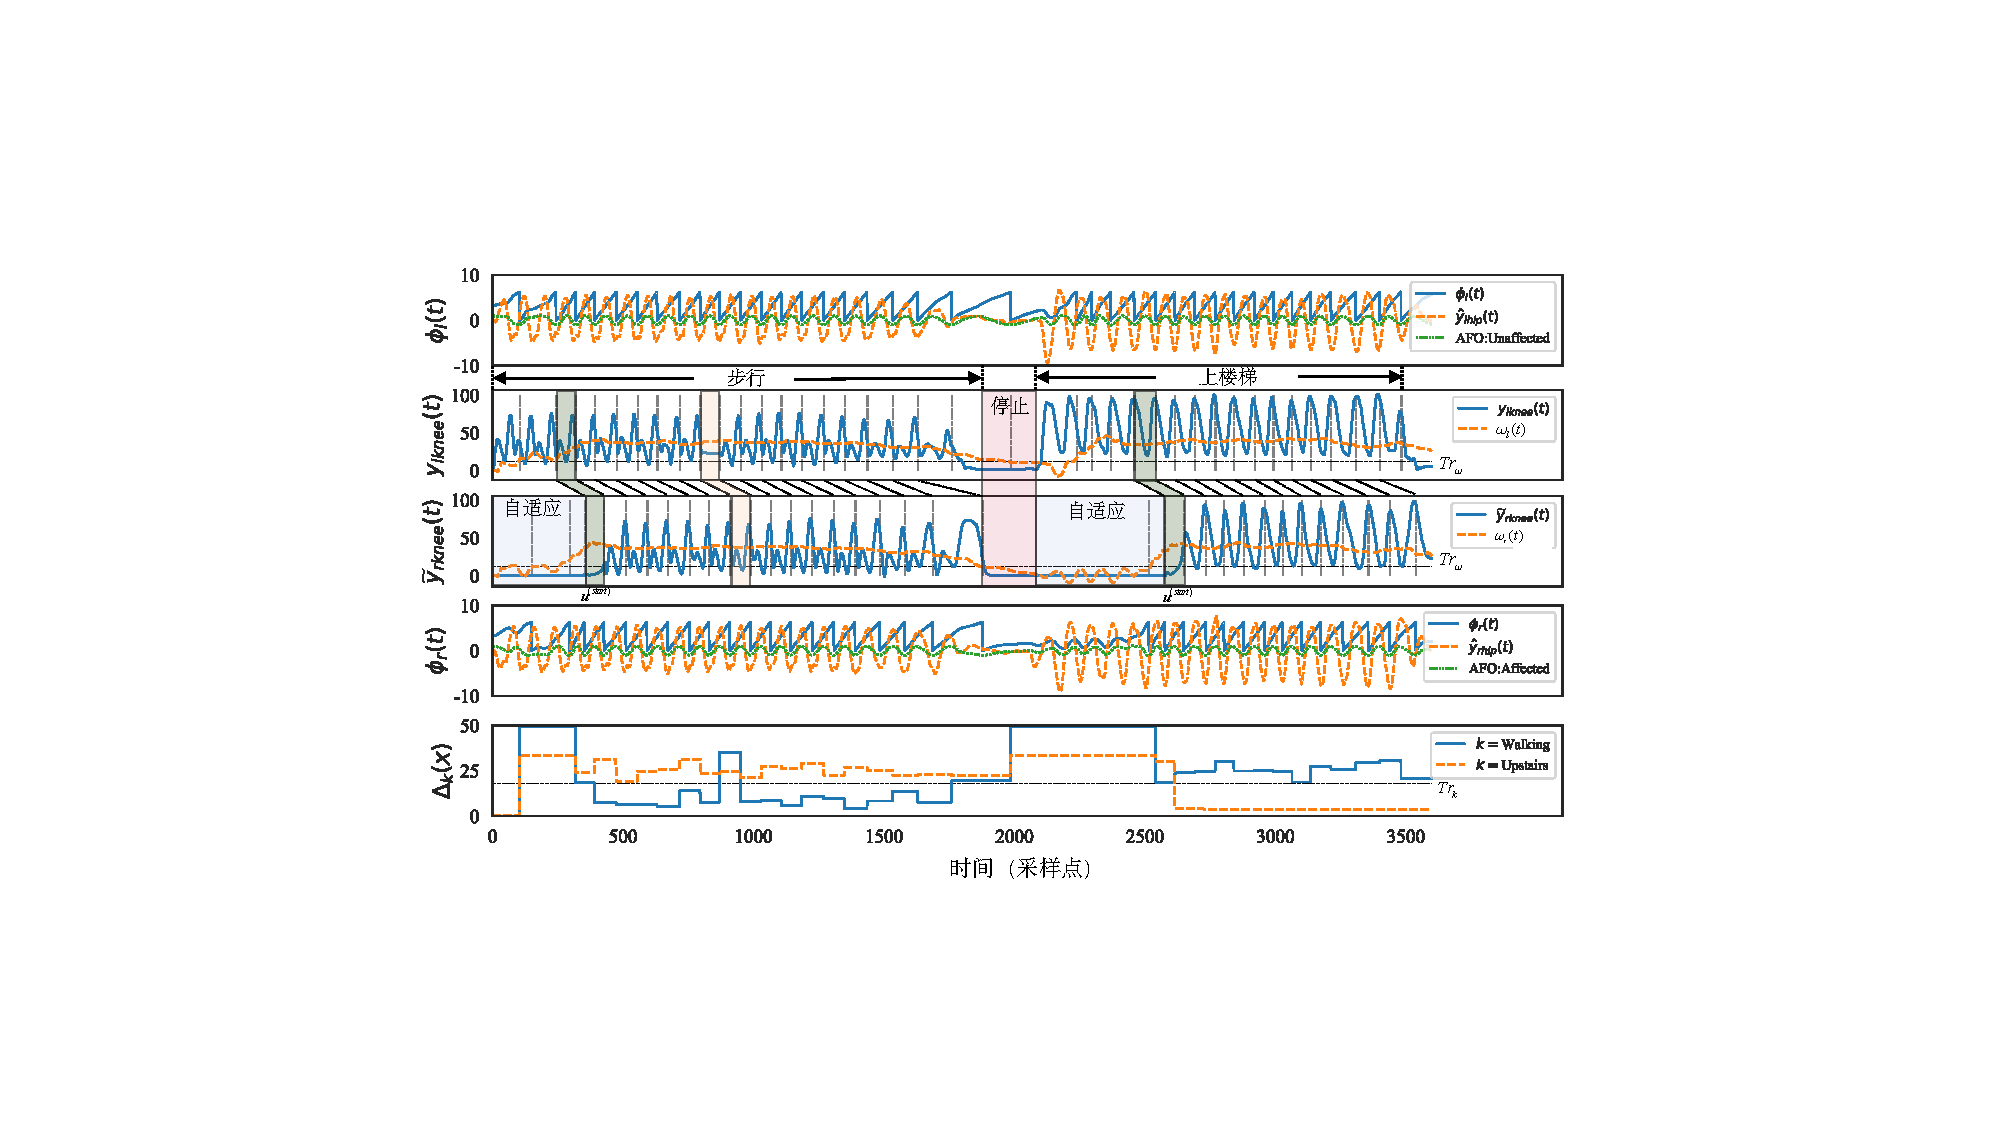
\includegraphics[width=1\textwidth]{figures/5-Fig-6.pdf}
  \caption{进行“行走”和“上楼梯”两种任务后生成的参考轨迹曲线,其中${\hat y_{lhip}}(t)$和${\hat y_{rhip}}(t)$是经过移动平均去趋势和 FIR低通滤波过后的髋关节角度曲线。}
  \label{fig:5-6}
\end{figure}

\subsection{主动式膝关节矫形器辅助步行实验}
为评估所提出框架在实际应用场景中的性能表现,我们招募了七名受试者,并邀请他们完成了四项不同的任务,每项任务重复三次。(``Normal'':不佩戴主动膝关节矫形器和沙袋行走;``Affected'':右脚踝上佩戴3公斤沙袋行走;``Assisted'':右脚踝上同时佩戴3公斤沙袋和主动膝关节矫形器行走; ``ThighLoad'':右大腿佩戴3公斤重的沙袋,在跑步机上以0.5公里/小时的稳定速度行走2分钟。其中,任务``ThighLoad''用于测试主动式膝关节矫形器自身重量(约 2.76 公斤)对步态对称性的影响。在图\ref{fig:5-7}中给出了实验结果,并基于单因素方差分析进行了统计分析。
\begin{figure}[htb]
  \centering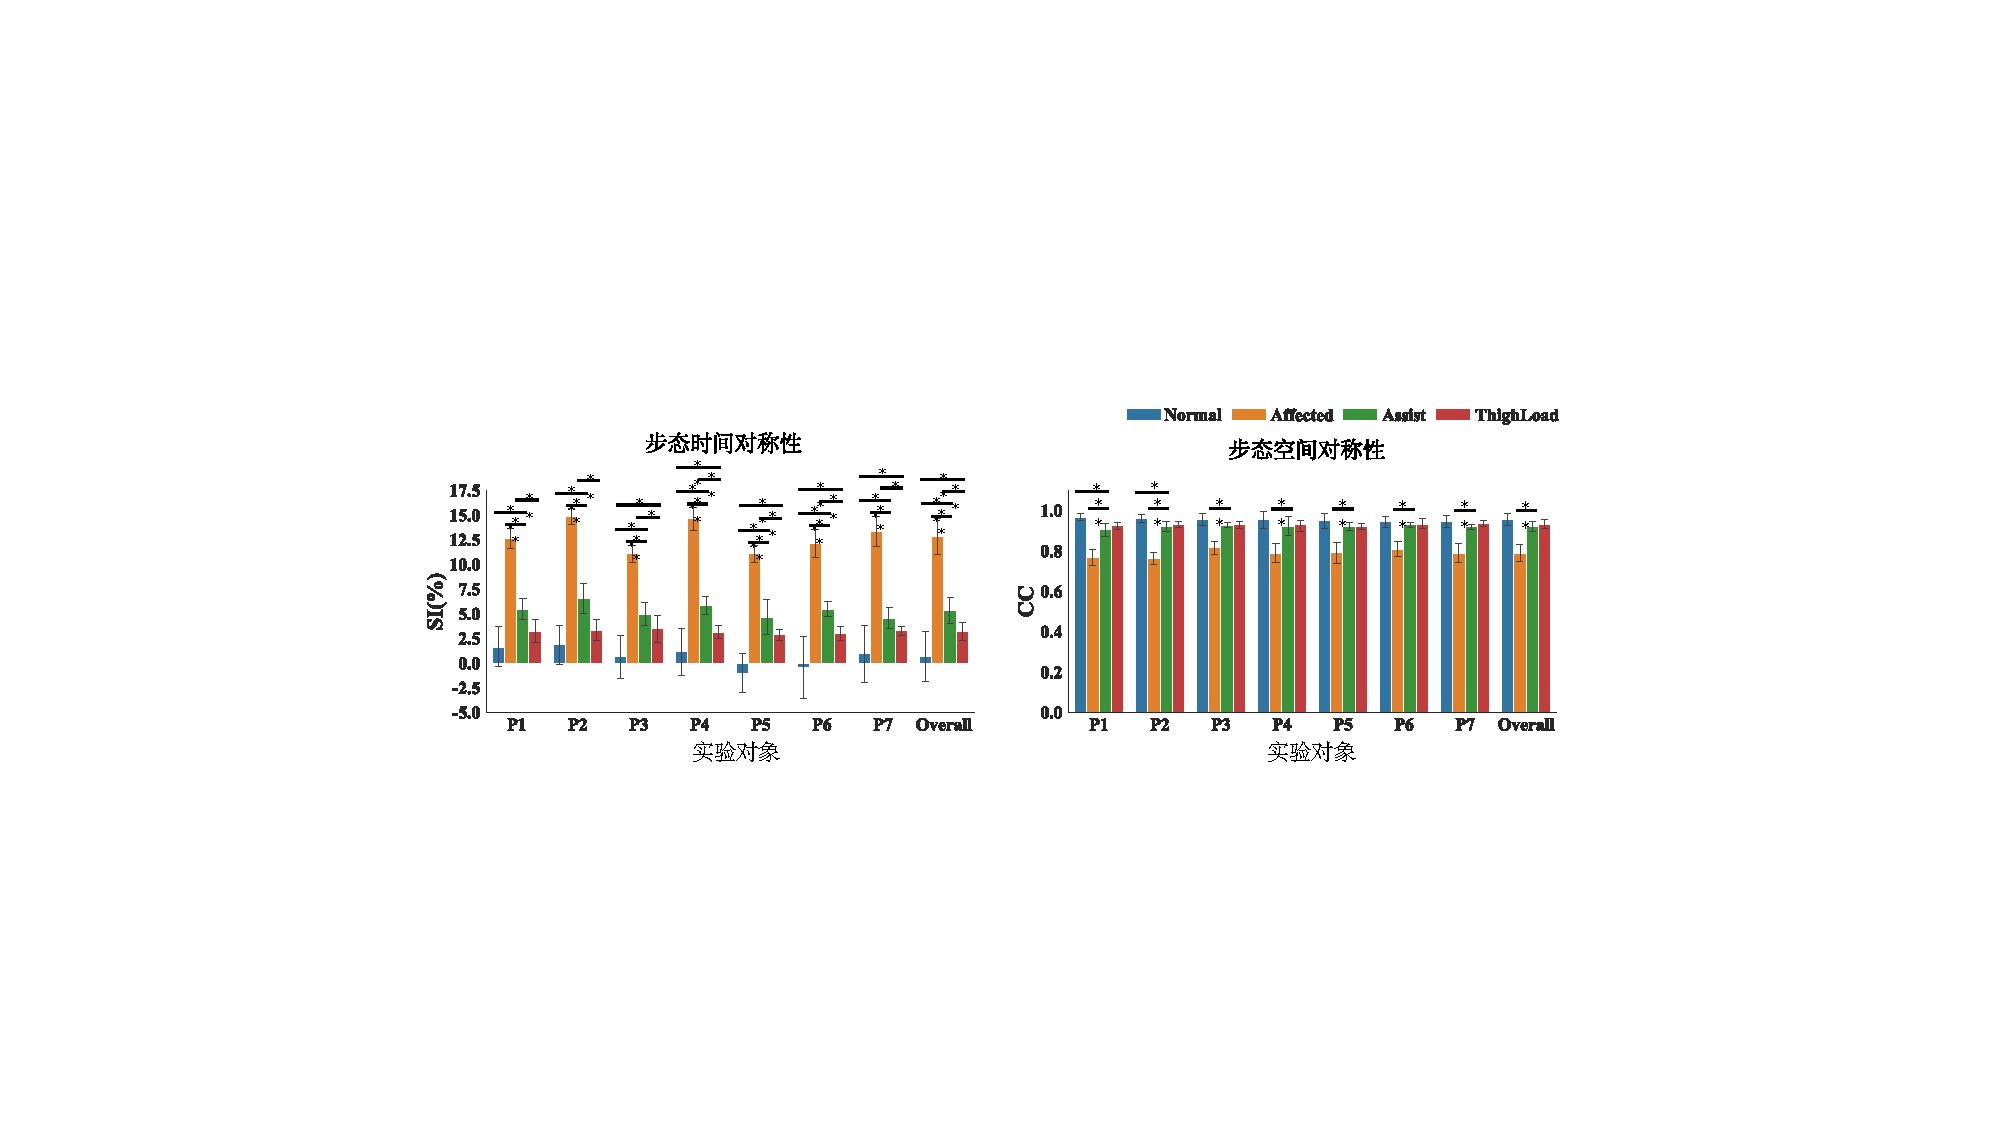
\includegraphics[width=1\textwidth]{figures/5-Fig-7.pdf}
  \caption{七名受试者使用主动式膝关节矫形器进行步行实验的对称性度量,图中的误差线为标准差,``*''代表$p \less 0.05$,``**''代表$p \less 0.01$}
  \label{fig:5-7}
\end{figure}

正常步态在时间和空间上通常呈现出对称性。这意味着在行走过程中,左右腿的动作在时间顺序、力量分布以及空间轨迹等方面具有高度的一致性。在步态对称性指标上一般表现为${SI < 6 \%}$和${CC}\approx {1}$\cite{balabanGaitDisturbancesPatients2014}。在实验中,我们发现附着在脚踝上的配重显著影响了所有受试者的步态时间对称性和空间对称性($p<0.01$),其中时间对称性指标达到平均${SI}=12.83 \%$,步态空间对称性下降到了平均${CC} = 0.79$。借助主动式膝关节矫形器的辅助,所有受试者的步态对称性均得到了一定程度的改善。其中``Affected''和``Assist''实验之间的步态时间对称性平均提高了约57 \% 至${SI} = 5.35 \%$,空间对称性平均提高了约17\%至${CC} = 0.94$。在所有受试者中,在``Assist''实验中的空间对称性虽然比``Affected''有所改善,但与``Normal''($p<0.01$)相比仍然显示出显著的变异性,这可能是由于所开发的主动矫形器的额外重量所导致的。此外,参与者P1和P2在``Normal''($p<0.05$)实验中相比``Assist''在步态空间对称性上表现出显著差异。

在``ThighLoad''实验中,位于大腿上的沙袋负重对受试者的步态时间对称性产生了显著影响,与``Normal''($p<0.01$)实验中的数据相比,它平均增加到了${SI}=3.22 \%$,但没有显着改变空间对称性。然而,``ThighLoad''和``Assist''之间的步态时间对称性仍然存在显著差异($p<0.01$)。因此,设备的自重可能并非步态时间对称性无法完全恢复的唯一因素。另一个潜在原因是,当前开发的主动式矫形器主要依赖于位置控制,导致交互透明性较差。然而,由于用于计算对称性的方程式和矫形器设计存在差异,对称性数值仍难以在不同研究间进行直接比较。在未来,将当前研究进一步改进控制策略以实现力-位置混合控制,并减轻所设计辅助设备的重量,对于推动进一步研究工作具有重要意义。

% 尽管如此,提供扭矩辅助的矫形器在恢复步态时间对称性方面已展现出与所提出方法相当的性能。但值得注意的是,其中大多数方法并未充分考虑下肢双侧关节运动角度的对称性。此外,由于采用串联弹性执行器和绳驱动结构,扭矩辅助主动矫形器仅能控制执行器输出力,从而提高了物理人机交互透明度。在未来,将当前研究进一步改进控制策略以实现力-位置混合控制,并减轻所设计辅助设备的重量,对于推动进一步研究工作具有重要意义。尽管已通过各种实验验证了该方法的有效性,但其仍存在一些局限性。例如,所提出的系统可能无法使患者完全恢复步态对称性,且可能不适用于下肢严重损伤的患者。在未来,围绕该系统我们计划在以下几个方面进一步展开工作:(1)招募偏瘫患者参与实验,收集更多运动数据以构建步态技能库;(2)在算法框架中引入力触觉传感器,并构建超参数$\theta$的人在环中优化算法。

\section{本章小结}
在本章中,围绕一个用于偏瘫患者步态对称性康复训练的主动式膝关节矫形器原型样机,详细地介绍了一种在线对称步态轨迹生成方法。此框架融合了节律性动态运动基元与自适应频率振荡器,实现了在线步态周期轨迹的编码与解码,同时实现了下肢健侧和患侧的步态相位自适应延迟。此外,通过离线任务采集数据,研究还设计了一个带有高斯先验步态技能库的共享自主模块,以自适应地分析和仲裁来自未受影响侧的实时用户输入,从而最大程度地减轻使用者健侧交互输入不确定性的影响。所提出的方法具有在非结构化或半结构化环境中实现步态对称性康复的潜力,并为关节扭矩辅助的主动式膝关节矫形器提供运动学参考。尽管已通过各种实验验证了该方法的有效性,但其仍存在一些局限性。例如,所提出的系统可能无法使患者完全恢复步态对称性,且可能不适用于下肢严重损伤的患者。在未来,围绕该系统我们计划在以下几个方面进一步展开工作:(1)招募偏瘫患者参与实验,收集更多运动数据以构建步态技能库;(2)在算法框架中引入力触觉传感器,并构建超参数$\theta$的人在环中优化算法。